% =====================================================================
%  main_en.tex  --  ENGLISH DRAFT (translated from the approved
%  Vietnamese source main.tex / body.tex)
%
%  Translation in progress: see body_en.tex for section-by-section
%  status. Do not treat as final until all sections are translated,
%  reconciled, and the semantic-regression check (PASS 7) is done.
%
%  Compile with: cd paper && tectonic -X compile main_en.tex
% =====================================================================
\documentclass[11pt,a4paper]{article}
\raggedbottom  % khong ep gian dong de lap day trang khi mot hinh/bang
               % bi day sang trang sau (tranh khoang trang lon giua trang)
% Noi long tham so dat bang/hinh mac dinh cua LaTeX (mac dinh qua chat,
% de khien nhieu bang/hinh bi day don thanh mot cum xa doan van tham
% chieu, tao khoang trang lon giua chung).
\renewcommand{\topfraction}{0.9}
\renewcommand{\bottomfraction}{0.8}
\renewcommand{\textfraction}{0.07}
\renewcommand{\floatpagefraction}{0.7}
\setcounter{topnumber}{4}
\setcounter{bottomnumber}{2}
\setcounter{totalnumber}{6}

% --- Fonts -------------------------------------------------------------
\usepackage{fontspec}
\setmainfont{TeX Gyre Termes}

% --- Page ---------------------------------------------------------------
\usepackage[margin=2.5cm]{geometry}
\usepackage{setspace}
\onehalfspacing

% --- Math ----------------------------------------------------------------
\usepackage{amsmath,amssymb}
\usepackage{braket}          % \ket{} \braket{}

% --- Tables, figures -------------------------------------------------------
\usepackage{booktabs}
\usepackage{multirow}
\usepackage{longtable}
\usepackage{array}
\usepackage{calc}
\usepackage{graphicx}
\graphicspath{{figs/}}
\usepackage{float}
\usepackage[section]{placeins}

% --- TikZ diagram (Figure 1) ----------------------------------------------
\usepackage[dvipsnames]{xcolor}  % load before tikz to avoid "option clash"
\usepackage{tikz}
\usetikzlibrary{arrows.meta,positioning,shapes.geometric,calc,decorations.pathmorphing,backgrounds,fit}

% --- Links, citations ------------------------------------------------------
\usepackage{hyperref}
\hypersetup{
    colorlinks=true,
    linkcolor=RoyalBlue,
    citecolor=RoyalBlue,
    urlcolor=RoyalBlue,
    }
\usepackage{cite}

\title{A Controlled Multi-Seed Evaluation of Relational Knowledge Distillation for Motor Imagery Decoding with Classical and Quantum Kernels}
\author{%
Duong Thi Mai Thuong$^{1}$, Nguyen Phuong Huy$^{2,\ast}$\\[4pt]
\small $^{1}$Department of Computer Science, Faculty of Information Technology, Thai Nguyen University of Information and Communication Technology, Thai Nguyen, Vietnam\\
\small $^{2}$Department of Electronics Engineering, Faculty of Electronics Engineering, Thai Nguyen University of Technology, Thai Nguyen, Vietnam\\
\small $^{\ast}$Corresponding author: \href{mailto:nguyenphuonghuy@tnut.edu.vn}{nguyenphuonghuy@tnut.edu.vn}\\
\small $^{1}$ORCID: \href{https://orcid.org/0009-0005-7862-7473}{0009-0005-7862-7473};
$^{2}$ORCID: \href{https://orcid.org/0000-0002-5887-5796}{0000-0002-5887-5796}
}
\date{}

\begin{document}
\maketitle

\begin{abstract}
\noindent
Knowledge distillation can transfer the accuracy of large motor imagery
decoders to compact networks for embedded brain--computer interfaces.
However, distillation mechanisms are usually compared from a single
training run, so their rankings may reflect training noise. The research contribution is
a controlled multi-seed evaluation protocol for these mechanisms, together
with quantitative evidence that seed noise exceeds the differences among
them. A structured relational distillation framework varies the
relation-formation strategy and the similarity kernel, classical or
quantum, with all other components fixed. Twelve mechanisms were evaluated
on PhysionetMI (103 subjects) with subject-wise cross-validation, five fixed
seeds, and a statistical plan fixed before running. In this confirmatory
analysis, distillation with a 30-epoch budget raised accuracy from 74.93\%
to 81.49\%, and an exploratory replication on Cho2017 (49 subjects) agreed
in direction. Beyond this gain, no relation strategy or kernel separated
significantly from logit-level distillation. The spread among mechanisms
(0.46 percentage points) was smaller than seed noise (0.75 points), and
single-run rankings were almost uncorrelated with five-seed rankings
(Spearman $\rho = 0.14$). The quantum kernel did not differ significantly
from cosine or RBF kernels, even with gradient-matched weighting, but these
data cannot establish equivalence. A factorial experiment crossing the two
design axes detected no interaction between them. The quantum branch exists
only during training, so the deployed student runs unchanged on a Raspberry
Pi 4, at about 13 times the training cost. Mechanism-level claims in
electroencephalography distillation should therefore rest on multi-seed
comparisons with confidence intervals.
\end{abstract}

\noindent\textbf{Keywords:} Brain--computer interface; knowledge distillation; motor imagery decoding; quantum kernel; reproducibility.

% =====================================================================
%  body_en.tex -- ENGLISH TRANSLATION IN PROGRESS
%  Status: Section 1 (Introduction) done.
%  Sections 2-5 (Related Work, Method, Experiments/Results, Conclusion):
%  not yet translated.
% =====================================================================

\section{Introduction}
\label{sec:gioithieu}

A brain--computer interface (BCI) converts electrical brain activity
into control signals for external devices without going through the
usual neuromuscular pathway \cite{chen2025brain, tonin2021noninvasive,
ding2026brain}. For people who have lost motor function, this is a
viable means of operating assistive devices. The scope of BCI
applications has expanded from the laboratory to many real-world
systems \cite{varbu2022present, pang2024applications}: electric
wheelchairs \cite{palumbo2021motorimagery, lei2022intention,
mai2024hybrid}, assistive robotic arms and prosthetic limbs
\cite{casey2021bci}, upper-limb rehabilitation devices
\cite{baniqued2021brain}, and intention-operated mobility vehicles
\cite{lu2020model}. Among the signal paradigms available for these
systems, this study focuses on motor imagery (MI).

In all the systems mentioned above, the EEG decoder does not operate
in isolation but is a link in a closed control loop. The user's
intent is converted into a command. The command is then executed by
the actuator. Finally, the outcome returns to the user as feedback.
This position imposes on the decoder requirements that a pure
classification problem does not consider. Inference time must fall
within the time budget of the closed loop, because accumulated
latency degrades the user's ability to make corrections
\cite{an2024development, tonin2020role}. Computational resources are
limited by the embedded hardware built into the device rather than a
workstation with a discrete GPU \cite{wang2024mibminet,
sun2025signal, craighero2024ondevice}. The strictest requirement is
reliability, particularly in systems that share control authority
with an autonomous mechanism \cite{choi2023asynchronous,
deng2020selfadaptive}. The BCI community quantifies the bandwidth of
the control channel using information transfer rate, a metric that
jointly combines accuracy and command time \cite{wolpaw2002brain}.

These constraints become more severe when the system moves to
consumer-grade devices with a low channel count, forcing the decoder
to achieve higher accuracy on poorer data while still running on
limited hardware.

Deep learning methods have substantially improved the quality of
motor imagery decoding compared with pipelines based on hand-crafted
features. Even so, the literature currently splits into two opposing
branches in terms of implementation. One branch consists of
lightweight architectures designed specifically for EEG, capable of
running on a microcontroller. The other branch consists of
large-capacity models that achieve higher accuracy but far exceed the
computational budget of the control loop. Designers therefore face a
choice between a decoder that is deployable but less accurate and a
decoder that is accurate but cannot be brought into the control loop.

Knowledge distillation is a strategy that directly targets this
conflict, allowing part of the capacity of a large-capacity model to
be transferred to a lightweight model without changing the inference
cost \cite{hinton2015distilling, gou2021knowledge, li2025lightweight}.
Among the forms of transferable knowledge, relations among samples
appear particularly well suited to EEG signals, where discriminative
information often lies in the relative structure among samples rather
than the absolute value of each sample \cite{park2019relational,
gou2025neighborhood}. Recent studies have applied this principle to
EEG, ranging from preserving similarity structure when moving to
low-electrode-density systems \cite{huang2024enhancing} to
multi-level distillation frameworks for motor imagery
\cite{wu2026multilevel, mai2025eegskdnet}.

Training a deep neural network is subject to multiple sources of
randomness, from weight initialization to mini-batch sampling order.
This effect can be substantially larger on small EEG datasets than on
vision or language data. Does the method ranking obtained from a
single training run correctly reflect the true difference among
distillation mechanisms, or does it merely reflect the noise specific
to that run? This is a question that is rarely measured directly in
the EEG distillation literature. If seed noise is larger than the
difference among mechanisms, a conclusion that ``method A is better
than method B'' drawn from a single run may reflect only the random
factor of that run rather than a real difference.

In parallel, quantum machine learning provides an alternative
representation space, in which data are mapped into a
high-dimensional Hilbert space and the relation among samples is
described by a quantum kernel function \cite{schuld2019quantum}. This
direction has been tested on EEG signals through hybrid backbones
\cite{chen2024qeegnet, chen2026exploring, olvera2024eegbased}. The
limitation is that the quantum component usually lies within the
inference pipeline. The deployed model must then access quantum
hardware or a simulator at runtime, which directly conflicts with the
real-time constraints noted above. Some recent work has moved the
quantum component to the training stage \cite{liu2025quantum,
liu2025quantumtrain}. This direction has not yet been verified on the
motor imagery decoding problem under control-loop constraints.

This study proposes a structured relational distillation framework
(QRD) for motor imagery decoders in brain-signal control systems. The
central idea is to separate the relation-formation strategy among
samples from the representation space used to measure relational
similarity, treating both as two independent design parameters
instead of tying them together as in prior work. In this study, the
representation space is investigated by encoding the intermediate
representations of the teacher and of the student into quantum
states through a parametrized circuit, compared directly against two
classical nonlinear kernel functions. The similarity between any two
samples is measured by the fidelity between their corresponding
states, forming a relation matrix for each model. The discrepancy
between the teacher's and the student's relation matrices becomes an
additional loss term, forcing the student to reproduce the relation
structure that the teacher has learned instead of merely matching
individual predictions. The entire relation kernel function, whether
classical or quantum, participates only in computing the loss
function and therefore disappears completely once training ends. The
model deployed into the control loop remains a lightweight classical
network.

What distinguishes QRD from existing relational distillation methods
does not lie solely in the representation space. In prior work, the
set of sample pairs used to construct relations is typically taken as
the entire mini-batch by default. QRD treats the way sample pairs are
selected, that is, the relation-formation strategy, as an independent
design parameter. On the same loss function, QRD investigates five
different relation-formation strategies, ranging from dense
relations, to sparse relations based on representative samples, to
guided selection based on the teacher's uncertainty level. By keeping
every remaining component fixed across variants, the effect of the
representation space can be separated from the effect of the relation
structure. Existing designs do not allow these two effects to be
separated because the two factors always change together.

On this basis, the paper makes the following three contributions.

\begin{itemize}
\item The paper surveys five relation-formation strategies and three
kernel function types within the same design space, directly
measuring the noise from random seeds and the difference among
distillation mechanisms. Seed noise (standard deviation about 0.75
percentage points) is larger than the difference among methods (about
0.46 percentage points). The method ranking from a single run is
almost uncorrelated with the ranking over five independent seeds,
with a Spearman coefficient of only 0.14. This is quantitative
evidence for a methodological risk that is rarely measured directly
in the knowledge distillation literature for EEG.

\item To produce this evidence under tightly controlled conditions,
the paper builds the QRD framework. This framework separates the
strategy for selecting sample pairs used to construct relations from
the representation space used to measure similarity, comprising a
classical kernel and a quantum kernel that lie outside the inference
pipeline. These two axes vary independently. Every other component is
kept fixed. Using the QRD framework, the paper confirms that
knowledge distillation in general provides a large and stable
benefit. This result is replicated on two independent datasets,
PhysionetMI and Cho2017. However, no specific relation variant or
kernel function, including the quantum kernel function, separates
from the KDBase baseline at a statistically significant level.

\item The paper proposes a control-oriented evaluation procedure,
using information transfer rate and the inference-time budget instead
of classification accuracy alone. This procedure is applied
consistently across every configuration in the survey framework and
is illustrated with a real inference-time measurement on embedded
hardware.
\end{itemize}

The remainder of the paper is organized as follows.
Section~\ref{sec:lienquan} surveys related research directions and
positions this study. Section~\ref{sec:phuongphap} presents the QRD
framework and its variants. Section~\ref{sec:thucnghiem} describes
the experimental setup and analyzes the results.
Section~\ref{sec:ketluan} concludes and outlines directions for
future development.

\section{Related Work}
\label{sec:lienquan}

\subsection{Brain--computer interfaces in assistive-device and robot control}

Section~\ref{sec:gioithieu} noted three groups of BCI devices verified
in practice: electric wheelchairs, assistive robotic arms/prosthetic
limbs, and upper-limb rehabilitation devices \cite{varbu2022present}.
Among the signal paradigms used for these devices, motor imagery (MI)
holds a distinct position. Users issue commands actively without
depending on an external stimulus such as SSVEP or P300, making it
suitable for sustained continuous control tasks
\cite{palumbo2021motorimagery}.

Wheelchair control is the most widely studied application among
mobility-assistance devices \cite{palumbo2021motorimagery}. Even so,
systems based solely on MI face reliability limits as the number of
commands to be distinguished increases. The literature addresses this
in two different ways. One approach adds another signal paradigm to
increase the number of available commands without reducing the
accuracy of each command \cite{mai2024hybrid}. The other approach
keeps the decoder unchanged but shares control authority with an
autonomous system, in which the BCI issues commands only at the level
of intent while trajectory tracking and obstacle avoidance are
handled by sensors \cite{choi2023asynchronous}. Both approaches
acknowledge the same reality that the quality of the decoder directly
determines the degree of intervention required from the supporting
layers behind it.

For the group of manipulation and rehabilitation devices, the
requirements placed on the decoder differ somewhat. Assistive robotic
arm and hand-exoskeleton systems typically operate in a loop with
direct visual feedback, so a wrong command not only reduces
effectiveness but also affects the user's training process
\cite{casey2021bci, baniqued2021brain}. When moving from offline
classification to real-time control, the response-time constraint
becomes the decisive factor for usability, even when offline accuracy
has already reached an acceptable level. This is consistent with the
observation of An et al. \cite{an2024development}.

One development direction is the shift from multi-channel
medical-grade EEG devices to consumer-grade devices with a low
channel count, in order to reduce cost and setup time for the end
user \cite{wu2022deepbrain}. Tarara et al. \cite{tarara2025motor}
investigated multi-class control capability on a 14-channel device
and showed that the limited channel count substantially narrows the
space of commands that can be reliably distinguished. A similar trend
also appears in input interfaces based on motor imagery, where deep
learning models are used to compensate for lower signal quality
\cite{paneru2025eeg}. This shift places the decoder in a position
where it must achieve higher accuracy on poorer data while still
being able to run on the limited hardware built into the device.

Therefore, the literature on applied BCI shows that the EEG decoder
is not an independent classifier but a link in a control loop,
subject to three constraints that a pure classification problem does
not consider: response time must fall within the budget of the
closed loop \cite{an2024development}, computational resources must
match the embedded hardware built into the device
\cite{wu2022deepbrain}, and command reliability must be stable
\cite{choi2023asynchronous}. These three constraints are usually
stated only in qualitative form, whereas comparing decoders requires
them to be represented by measurable quantities.

\subsection{Real-time constraints and embedded deployment in the BCI control loop}
\label{sec:rangbuoc}
When the EEG decoder is placed into a control loop, classification
accuracy is no longer a sufficient quantity to describe system
quality. The BCI community has long used information transfer rate
(ITR) to measure the bandwidth of the control channel, in which
accuracy and command time are combined into a single metric
\cite{wolpaw2002brain}. For an $N$-class problem with accuracy $P$,
the amount of information obtained per command is

\begin{equation}
\label{eq:itr-bits}
B = \log_2 N + P\log_2 P + (1-P)\log_2\!\left(\frac{1-P}{N-1}\right),
\end{equation}

and the information transfer rate in bits per minute is

\begin{equation}
\label{eq:itr-rate}
\mathrm{ITR} = B \times \frac{60}{T},
\end{equation}

where $T$ is the time required for one command, in seconds. For the
two-class case, expression \eqref{eq:itr-bits} reduces to
$B = 1 - H(P)$, where $H$ is the binary entropy function. This
nonlinear relationship has a consequence for design. In the
mid-accuracy range, a small improvement in accuracy produces a
bandwidth gain much larger than the corresponding ratio. ITR computed
via \eqref{eq:itr-rate} relies on several assumptions about operating
conditions. Applying it carelessly in online systems can lead to
biased estimates \cite{yuan2013study}.

The time $T$ in \eqref{eq:itr-rate} does not consist solely of the
signal window length. In a real operating system, the time budget of
the closed loop is decomposed as

\begin{equation}
\label{eq:latency}
T_{\mathrm{loop}} = T_{\mathrm{window}} + T_{\mathrm{infer}}
                  + T_{\mathrm{command}},
\end{equation}

where $T_{\mathrm{window}}$ is the length of the signal segment to be
acquired, $T_{\mathrm{infer}}$ is the model's inference time, and
$T_{\mathrm{command}}$ is the time to transmit and execute the
command on the actuator. The second component is the only one that
model design can directly affect, and it is also the component most
often neglected in offline evaluation studies.

The constraint on $T_{\mathrm{infer}}$ becomes tighter when the
decoder is deployed on the hardware built into the device rather than
run on a workstation. This trend stems from three motivations:
reduced latency from not having to transmit data, protection of the
user's biological data, and increased system portability
\cite{sun2025signal}. Wang et al. \cite{wang2024mibminet} deployed a
convolutional network for motor imagery classification on an
ultra-low-power microcontroller, achieving an inference time on the
order of a few milliseconds with consumption of a few tens of
micro-joules per inference. This result shows that a sufficiently
lightweight decoder can meet real-time constraints on embedded
hardware, whereas large-capacity models cannot.

The requirement to deploy on a microcontroller imposes limits not
only on time but also on memory and energy. These limits need to be
considered jointly rather than separately \cite{akbari2025atrial,
craighero2024ondevice}. Available memory determines the maximum
number of parameters, the energy budget determines battery life, and
inference time determines the command rate. These three quantities
constrain one another, so a model that meets the requirement along
only one dimension while violating the other two still cannot be
deployed.

Besides speed, command reliability is the second evaluation dimension
that a pure classification problem does not consider. In a system
controlling an assistive device, the consequence of a wrong command
is not symmetric with the benefit of a correct command, because a
wrong command may require corrective action or pose a safety risk.
For this reason, Cohen's kappa coefficient is preferred over raw
accuracy in BCI evaluation because it corrects for chance agreement
and more closely reflects how trustworthy the issued command is. The
stability of reliability across sessions and across subjects is also
a practical issue. This motivates research directions aimed at
reducing the calibration effort required before use \cite{wei2023intra}.

The three quantities noted in the previous part can all be
quantified: control-channel bandwidth via \eqref{eq:itr-rate}, the
time budget via \eqref{eq:latency}, and command reliability via the
kappa coefficient. This paper uses all three as evaluation criteria
alongside classification accuracy. This allows decoder architectures
to be compared both by accuracy and by their ability to meet the
control loop's budget. However, the chance-correction advantage of
kappa only takes effect when the classes are imbalanced or number
more than two. For the balanced two-class problem examined here,
kappa is a deterministic linear transformation of accuracy
($\kappa = 2\,\mathrm{acc} - 1$) and carries no additional
information, as noted again in Section~\ref{sec:ketqua}.

\subsection{Deep learning decoders for motor imagery}

Motor imagery signal decoding has gradually shifted from pipelines
based on hand-crafted features to end-to-end deep learning models
\cite{al-saegh2021deep, sadiq2021development}. In these models, the
feature-extraction step and the classification step are optimized
jointly. This shift substantially improves accuracy but at the same
time gives rise to the design conflict noted in the previous parts.
The higher a model's representational capacity, the harder it is to
satisfy the constraints of the control loop.

One branch of the literature pursues lightweight architectures
designed specifically for EEG signals. EEGNet \cite{lawhern2018eegnet}
uses depthwise and separable convolutions to sharply reduce the
number of parameters while still preserving the spatio-temporal
structure specific to EEG, and it became the reference architecture
for most subsequent studies. Subsequent work extended it in two
directions: adding a temporal convolution module to capture longer
dependencies \cite{ingolfsson2020eegtcnet}, or refining the structure
and quantizing the weights to fit a microcontroller
\cite{wang2024mibminet}. Other variants focus on combining
frequency-domain or time--frequency-domain representations to
increase accuracy without substantially increasing computational cost
\cite{deng2021advanced, wang2022mieeg, wang2023ifnet}.

The other branch takes the opposite direction, increasing model
capacity to extract the maximum information from the signal. Deep
convolutional networks applied directly to raw EEG sequences have
shown the ability to learn physiologically meaningful features
\cite{schirrmeister2017deep}. Recently, transformer architectures
have been introduced into this field to model long-range dependencies
that convolution struggles to capture \cite{vafaei2025transformers}.
Many hybrid convolution--transformer variants have been proposed
\cite{zhao2024ctnet, ding2025eegdeformer, altaheri2025temporal}. In
these, the convolutional component handles local features while the
attention component handles global relations. Recurrent architectures
combined with convolution have also been explored in a similar
direction \cite{wang20232d}. Approaches that use an ensemble of
multiple models simultaneously push accuracy even higher, but
inference cost increases with the number of components
\cite{zoumpourlis2024motor}.

The difference between the two branches does not lie in accuracy
alone. Large-capacity models require substantially more training
data, whereas EEG data is inherently costly to collect and is limited
by how long a participant can sustain attention. Keutayeva and
Abibullaev \cite{keutayeva2024data} systematically investigated this
issue. The results show that the performance of transformer-based
models in BCI depends strongly on the amount of available data,
meaning that an advantage in representational capacity does not
always translate into a practical advantage.

The cross-subject generalization problem makes this conflict even
more acute. Because EEG characteristics vary strongly among
individuals, a model trained on one group of subjects often degrades
markedly when applied to a new subject. The traditional approach is
to calibrate separately for each user. This approach lengthens setup
time and reduces the usability of the system \cite{wei2023intra}.
Architectures aimed at subject-independent operation are attracting
considerable interest. Among these are lightweight transformer
variants that aim to balance generalization ability against
computational cost \cite{keutayeva2024compact}.

The current literature therefore places designers before a binary
choice. Lightweight models satisfy the deployment constraints noted
above but accept a lower level of accuracy. Large-capacity models
achieve higher accuracy but exceed the time and resource budget of
the control loop, while also depending more heavily on the amount of
available data. The question that arises is whether part of the
capacity of the large-capacity group can be transferred to the
lightweight group without carrying over its deployment cost.

\subsection{Knowledge distillation and relation-based distillation}
\label{sec:kd}

Knowledge distillation (KD) was originally proposed to compress
models by transferring knowledge from a teacher model to a smaller
student model, based on the soft prediction distributions at the
output layer \cite{hinton2015distilling}. This approach helps the
student learn the probabilistic structure among classes that hard
labels do not fully reflect. According to systematic surveys, KD
methods are currently classified into three main groups according to
the type of knowledge transferred: output-based, feature-based, and
based on relations among samples \cite{gou2021knowledge,mansourian2025comprehensive}.

The feature-based group transfers knowledge at intermediate
representation layers rather than only at the output. FitNets uses
hint information from the teacher's hidden layers to guide the
student's training \cite{romero2015fitnets}, while Attention Transfer
exploits attention maps as a more structured form of knowledge
\cite{zagoruyko2017paying}. The approach of supervising multiple
feature layers simultaneously has also been successfully applied to
biomedical imaging problems \cite{javed2023knowledge}.

The group based on relations among samples, which is closest to this
study, models knowledge through the relations among samples rather
than the attributes of each individual sample. Relational Knowledge
Distillation represents knowledge using geometric quantities such as
the distance and angle between representation vectors in feature
space \cite{park2019relational}. Subsequent variants exploit
different relation structures: relations based on pairwise similarity
\cite{feng2021double}, relations within the local neighborhood of
each sample \cite{gou2025neighborhood}, or relations built
recursively over multiple steps \cite{ye2021unsupervised}. The common
point of this group is the assumption that the relative structure
among samples carries discriminative information that the absolute
representation of each sample cannot express. The point that has not
been clarified is that the choice of which sample pairs to use for
constructing relations remains largely heuristic. The effect of this
choice has not been systematically investigated.

Another development branch is self-distillation. Knowledge is reused
directly during the model's own training process without requiring a
separate teacher \cite{zhang2019be}. In the EEG domain, EEG-SKDNet
\cite{mai2025eegskdnet} combines a self-distillation mechanism with
an adaptive weighting strategy to improve emotion-recognition
performance.

On physiological signals, KD is used with two parallel goals:
reducing model size and improving representation quality under
limited data conditions. Frame-level distillation frameworks have
been proposed for EEG-based emotion recognition \cite{wang2021fldnet,gu2023framelevel}.
In these frameworks, knowledge is transferred segment by segment in
time rather than over the entire sequence. The direction of
distilling representations through hierarchical structures has also
shown effectiveness on affective computing problems
\cite{zhang2023distilling}. Beyond EEG, KD has also been applied to
electronic medical record data \cite{ibrahim2022knowledge} and to
incremental learning problems on neural signals
\cite{garcia-salinas2023intrasubject}, showing the generality of this
methodological framework in the field of biological signals.

KD is one of the main strategies used to build lightweight EEG
decoders suitable for practical deployment, alongside directions such
as structural optimization and quantization \cite{li2025lightweight}.
KD retains part of the capacity of a large-capacity model within a
model whose inference cost is suited to the control loop.

In the EEG context, preserving the relation structure among samples
appears particularly well suited. Similarity-Keeping Knowledge
Distillation \cite{huang2024enhancing} preserves the similarity
structure among samples when transferring knowledge from a
high-electrode-density EEG system to a low-density system, thereby
improving the performance of practical BCI systems. Multi-level
distillation frameworks with a dynamic feedback mechanism have also
been proposed for the motor imagery problem \cite{wu2026multilevel}.
Knowledge in these frameworks is transferred across multiple levels
and adjusted adaptively during training.

These results show that relations among samples play an important
role in the effectiveness of distillation for the EEG problem.
However, all the studies noted above construct relations in a
classical metric space. The open question is whether the observed
limitation originates from the relation structure itself or from the
metric space used to measure it.

\subsection{Quantum machine learning for biological signals and EEG}
\label{sec:qml}

The theoretical basis of quantum machine learning in classification
problems lies in the observation that a parametrized quantum circuit
can be viewed as a mapping of classical data into a high-dimensional
Hilbert space. In this space, the inner product between two states
plays the role of a kernel function \cite{schuld2019quantum}. This
view places quantum machine learning within the same framework as
classical kernel-based methods, while also opening up the
possibility of constructing kernel functions that are hard to
compute efficiently with a classical computer. On this basis, many
classifier circuit structures have been proposed
\cite{schuld2020circuitcentric}. Parametrized rotation layers
alternating with entangling-gate layers create nonlinear
representational capacity. In practice, the extent to which these
structures can be exploited is still limited by the number of
available qubits, circuit depth, and the noise level of current
hardware \cite{xie2025advances}.

In the biomedical field, quantum machine learning has been
investigated on many different types of data, from medical images to
physiological signals, in the hope of exploiting the representational
capacity of Hilbert space under limited training data
\cite{idzikowski2026survey}. This characteristic makes the research
direction suited to EEG signals, which are costly to collect and have
a low signal-to-noise ratio.

For EEG signals, the most common direction is to integrate
parametrized quantum circuits into classical deep learning backbones.
QEEGNet extends the EEGNet architecture \cite{lawhern2018eegnet} by
inserting a quantum circuit into the feature-extraction process,
exploiting the nonlinear representation of Hilbert space in the
signal-encoding step \cite{chen2024qeegnet}. Subsequent studies
extended the evaluation to cross-task and cross-dataset scenarios,
showing that model effectiveness depends considerably on how the
quantum component is integrated as well as on the training
configuration \cite{chen2026exploring}.

Another group of studies places the quantum component at the end of
the processing pipeline, where features are extracted by a classical
network before being passed to a quantum or hybrid classifier
\cite{olvera2024eegbased}. This direction has also been applied to
BCI with classifiers combining quantum support vector machines and
quantum neural networks \cite{behera2026qsvmqnn}. More complex
architectures use multiple parallel branches, a representative
example being a dual quantum--classical branch convolutional network
for seizure detection \cite{dutta2026duoqepinet}. Recently, the
direction of differentiable quantum architecture search combined with
transfer learning has also been tested on EEG data
\cite{park2026qdiver}.

Similar design patterns appear in many other application fields, from
image recognition \cite{wang2022development} to weak-signal detection
\cite{griol-barres2021variational}, as well as in end-to-end learning
frameworks combining tensor networks with variational quantum
circuits \cite{qi2024qtnvqc}. The common point across this entire
group of studies is that the quantum component is placed directly
within the model's inference pipeline.

This is precisely the point at which the current study departs from
the direction above. When the quantum circuit lies within the
inference pipeline, the deployed model must access quantum hardware
or a simulator at runtime. This directly conflicts with the latency
and resource constraints noted above. This study does not propose a
new quantum EEG backbone. Instead, the quantum component participates
only in the training stage, in the role of modeling relations among
samples, while the deployed model is an entirely classical network.
As a result, the benefit of the quantum representation space is
retained without carrying over its deployment cost.

\subsection{Knowledge distillation in the quantum setting}
\label{sec:qkd}

Knowledge distillation has recently been extended to the field of
quantum computing, reflecting the trend of combining classical deep
learning with quantum models. Studies in this direction can be
grouped according to the role of the teacher, the student, and the
quantum component within the overall processing pipeline.

The first group uses distillation to compress quantum models
themselves. Both the teacher and the student are quantum neural
networks \cite{yan2026distilling}. The motivation for this direction
stems from the practical limitations of current hardware, where the
number of qubits and circuit depth are tightly constrained, and noise
degrades inference quality \cite{alam2022qnet}. At distributed scale,
distillation has also been used to synchronize multiple quantum
models trained in parallel \cite{oh2025quantum}. The infidelity
between states serves as the guiding signal in this synchronization
process.

The second group transfers knowledge from a classical model to a
quantum model, with the teacher being a deep learning network and the
student being a smaller quantum model \cite{nishan2026quantummedkd,
li2025quantum}. The reverse direction has also been investigated, in
which a classical neural network learns to emulate quantum dynamics
through a distillation mechanism \cite{yao2023emulating}. The common
point of both groups above is that the quantum component is still
present in the final inference model.

The third group, and also the group closest to this study, uses
quantum computing as a supporting tool during training rather than
as a component of the deployed model. Quantum Relational Knowledge
Distillation \cite{liu2025quantum} maps the intermediate
representations of the teacher and student into a quantum space,
then models the relations among samples through a quantum kernel
function. In this setup, both the teacher and the student are
classical models, while the quantum component participates only in
constructing the loss function. Following the same philosophy,
Quantum-Train \cite{liu2025quantumtrain} uses a quantum circuit
during training to reduce the number of trainable parameters of a
classical network, achieving competitive performance at a
substantially lower parameter cost. The theoretical basis for these
directions lies in the fact that a quantum kernel function can
describe the relation among representations in a way that differs
from a classical kernel function \cite{liu2022representation}.

This approach has an important advantage for systems subject to
deployment constraints. It exploits the quantum representation space
without introducing any quantum cost into the inference pipeline.
For an EEG decoder operating within a control loop, this is a
necessary condition for the method to be practically applicable.

However, existing studies on quantum relational distillation have
mainly been developed and validated on computer vision or natural
language processing problems. When moving to EEG signals, which have
a low signal-to-noise ratio and vary strongly among individuals, the
effectiveness of this approach has not been verified. In addition,
the quantum relation loss usually appears only as a single component
within the distillation pipeline, with a fixed relation structure
chosen heuristically.

This raises a question that remains unanswered in the literature:
whether the observed effectiveness of quantum relational distillation
comes from the quantum representation space itself or from how
relations among samples are organized and selected. These two
factors always appear together in existing work and therefore cannot
be separated. Separating them requires a survey framework that
allows each factor to be varied independently while keeping the
remaining components fixed. This is precisely the starting point of
the QRD framework proposed in this study.

\subsection{Positioning of this study}
\label{sec:dinhvi}

The sections above show a gap at the intersection of three research
directions. The literature on applied BCI places the EEG decoder
within a control loop and imposes on it constraints on latency,
resources, and command reliability (Section~\ref{sec:rangbuoc}), but
most decoding studies still evaluate models using offline accuracy.
The literature on knowledge distillation provides tools to narrow the
gap between large-capacity models and deployable models
(Section~\ref{sec:kd}). The strategy for constructing relations among
samples there, however, is almost always fixed heuristically. The
literature on quantum machine learning proposes alternative
representation spaces (Sections~\ref{sec:qml} and~\ref{sec:qkd}). The
quantum component in those proposals, however, usually lies within
the inference pipeline, conflicting with the very deployment
constraints noted above.

Among the studies surveyed, four are closest to this study. Each
stops short at a different limitation. Similarity-Keeping Knowledge
Distillation \cite{huang2024enhancing} preserves the similarity
structure among samples when transferring knowledge to a
low-electrode-density EEG system, but the relations are constructed
in Euclidean feature space and according to a fixed strategy. The
multi-level distillation framework with dynamic feedback
\cite{wu2026multilevel} organizes knowledge transfer across multiple
levels for the motor imagery problem, but its focus is on the
hierarchy of knowledge transfer rather than on how relations among
samples are formed. In the quantum direction, Quantum Relational
Knowledge Distillation \cite{liu2025quantum} brings relations into
Hilbert space but has only been verified on vision and language
problems, where the noise characteristics and inter-individual
variation do not arise as they do with EEG signals. Quantum-Train
\cite{liu2025quantumtrain} keeps the quantum component entirely
outside the inference pipeline, consistent with the deployment
constraints noted in Section~\ref{sec:rangbuoc}. The quantum circuit
there is used to reduce the number of parameters rather than to model
relations among samples.

This study lies at the intersection of the four directions above,
with the core difference from all four works being that it treats
the strategy for constructing relations among samples as a variable
to be surveyed rather than a fixed design choice. As a result, the
effect of the representation space can be separated from the effect
of the relation structure. The representation space surveyed includes
both classical and quantum kernel functions, applied jointly to the
motor imagery decoding problem under the control-loop constraints
noted in Section~\ref{sec:rangbuoc}. The quantum part specifically
participates only in the training stage and disappears from the
deployed model, so it does not violate that constraint. The specific
contributions were presented in Section~\ref{sec:gioithieu}.

Besides the content gap noted above, there is also a gap in how
distillation mechanisms are compared with one another. Comparisons
among mechanisms, whether relation-based or not, are typically
reported from a single training run. In other fields, reporting only
a single score has been shown to be insufficient for comparing
non-deterministic methods. Picard \cite{picard2021torch} showed that
changing the random seed alone can produce a substantial accuracy
difference between training runs of the same computer vision
architecture. Bouthillier et al. \cite{bouthillier2021accounting}
argued that many sources of variation, not just the seed, need to be
accounted for when comparing machine learning methods in order to
avoid biased conclusions. This issue has not been measured directly
in the knowledge distillation literature for EEG.

\section{Proposed Method}
\label{sec:phuongphap}

\subsection{Overview of the proposed method framework}

This part describes how the components of the QRD framework connect
to one another and defines the role of each component during
training. Figure~\ref{fig:khung} shows the entire architecture.

The framework is organized as a teacher--student setup. The teacher
is a pretrained ensemble model \cite{zoumpourlis2024motor}, kept
fixed and serving only as the source of the supervisory signal. The
student is an EEGNet network \cite{lawhern2018eegnet} and is the only
component in the teacher--student pair whose parameters are updated
\cite{hinton2015distilling}. The exception concerning the quantum
circuit shared between the two branches is discussed in
Section~\ref{sec:qrd}.

This pair of models was chosen to concretely realize the conflict
noted above. The ensemble model aggregates information from multiple
components and therefore provides a stable supervisory signal.
However, its memory and computational cost increases with the number
of components, making it poorly suited to the embedded hardware
built into the device. EEGNet, conversely, has a parameter count and
inference time suited to embedded hardware and has been verified in
practically deployed BCI systems \cite{wang2024mibminet}. The
performance gap between the two models is precisely the quantity
that the distillation framework seeks to narrow.

The supervisory signal delivered to the student consists of a base
component that matches the soft prediction distribution at the
logits level, plus at most one of three additional components
depending on the configuration. The general loss function for this
combination is written in \eqref{eq:total}, with the coefficients of
the components not belonging to the configuration under
consideration set to zero. The first two additional components
belong to classical distillation, comprising alignment of
intermediate features and preservation of the geometric structure
among samples in feature space. Both are presented in
Section~\ref{sec:cocdien} and used as the basis for comparison.

The third additional component is the quantum relation branch, the
contribution of this study. This branch takes the intermediate
features of both models, constructs a relation matrix in Hilbert
space, and produces an additional loss component. It exists only in
the computational graph of the training stage, does not appear in
the inference path, and therefore does not change the configuration
of the deployed model.

In terms of implementation, the relation matrix is not constructed
according to a single rule. Five different variants share the same
loss function and the same set of hyperparameters, differing in the
input index set. For the first four variants (V1--V4), this index
set is determined on the same position-fixed subsample, so the
difference observed among them reduces directly to how relations are
selected. The fifth variant (V5) not only changes how relations are
selected but also expands the candidate pool used for selection.
This additional difference, and how it affects the interpretation of
V5's results, is detailed in Section~\ref{sec:bienthe}.

\begin{figure}[H]
\centering
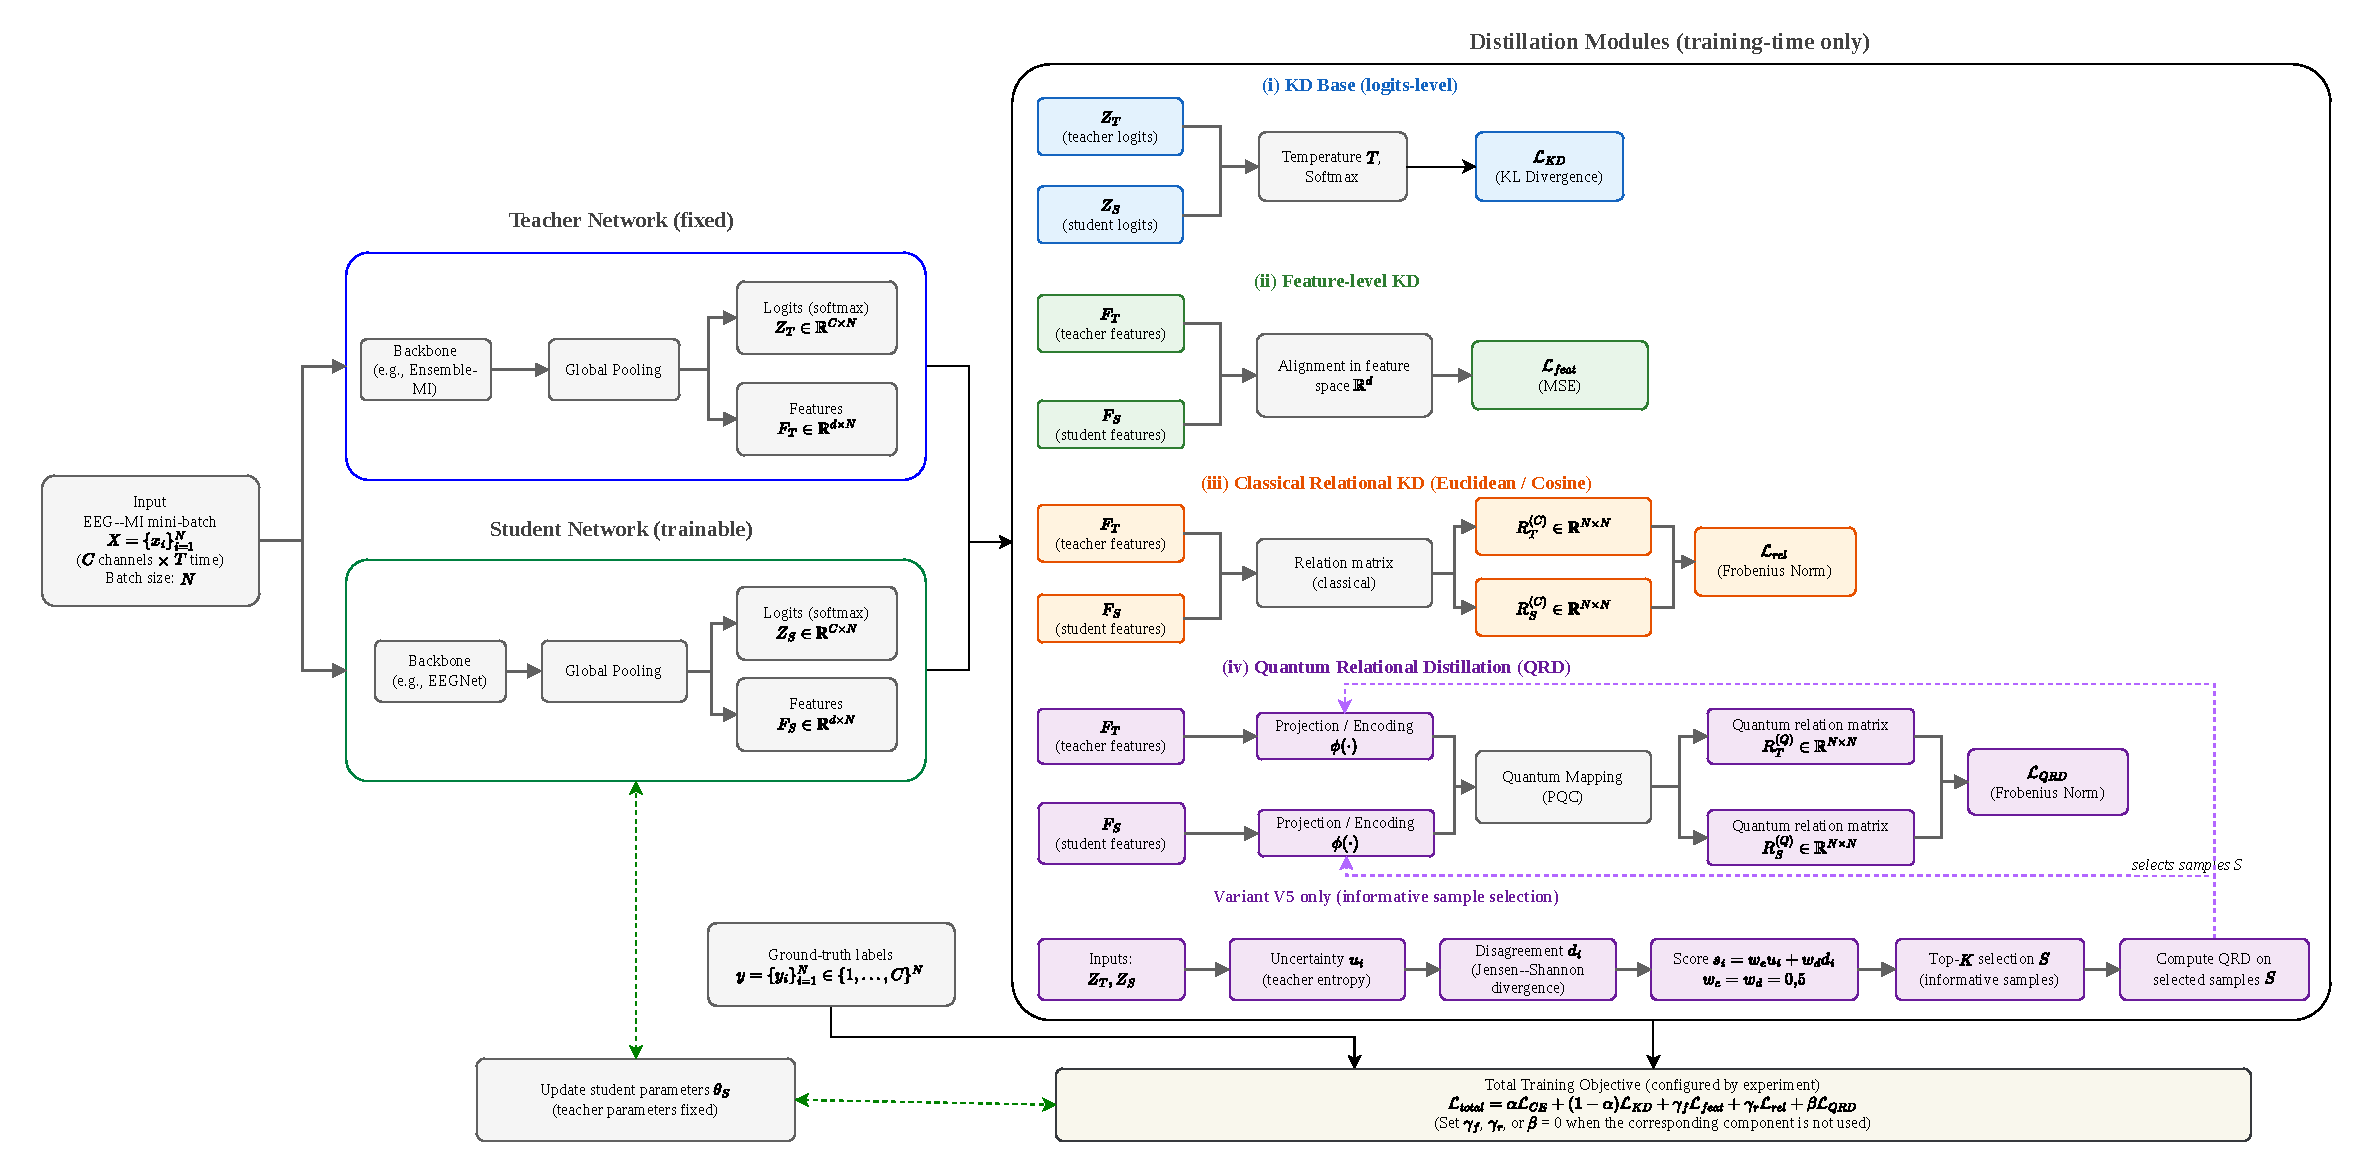
\includegraphics[width=\linewidth]{figs/fig12_QRD.drawio.pdf}
\caption{Overall teacher--student framework with the proposed
quantum relational distillation branch.}
\label{fig:khung}
\end{figure}
\FloatBarrier

The remainder of this part establishes the notation used
consistently throughout Section~\ref{sec:phuongphap}.
Consider a mini-batch of $N$ EEG samples $\{x_i\}_{i=1}^{N}$. For
each sample, each model produces two types of output: the logit
vectors $z_T(x_i), z_S(x_i) \in \mathbb{R}^{C}$ at the classification
layer, and the feature vectors $f_T(x_i), f_S(x_i) \in \mathbb{R}^{d}$
at the last representation layer before the classification layer.
For the pair of models used, $C = 2$ and $d = 144$ for both the
teacher and the student.

Stacking the feature vectors by column gives the feature matrix of
the mini-batch, matching the convention used in Figure~\ref{fig:khung}:

\begin{equation}
\label{eq:featmat}
F_T = \begin{bmatrix} f_T(x_1) & \cdots & f_T(x_N) \end{bmatrix}
\in \mathbb{R}^{d \times N},
\qquad
F_S = \begin{bmatrix} f_S(x_1) & \cdots & f_S(x_N) \end{bmatrix}
\in \mathbb{R}^{d \times N}.
\end{equation}

Distillation at the relational level does not compare $F_T$ with
$F_S$ directly but compares the relation structure among samples
within each model. This structure is represented by two symmetric
matrices $R_T$ and $R_S$, in which element $(i,j)$ measures the
similarity between two samples $x_i$ and $x_j$ according to the
representation of the corresponding model. In classical relational
distillation methods, these two matrices are constructed from
Euclidean distance or cosine similarity in feature space
\cite{park2019relational}. Section~\ref{sec:qrd} replaces that space
with a Hilbert space, in which similarity is measured by a quantum
kernel function.

The relation matrix is not necessarily computed over the entire
mini-batch. The set of participating index pairs, denoted
$\mathcal{I}$, is a configuration parameter and is defined
separately for each variant in Section~\ref{sec:bienthe}.

\subsection{Classical distillation setups}
\label{sec:cocdien}

This part defines three classical distillation configurations used
as baselines. All three share the same teacher, student, dataset,
and optimization protocol. The only component that changes is the
form of the additional supervisory signal. Because of this
constraint, any observed performance difference can be attributed to
the knowledge-transfer mechanism.

\textbf{KDBase} performs distillation at the output level, matching
the student's soft prediction distribution to the teacher's through
temperature-softened Kullback--Leibler divergence
\cite{hinton2015distilling}:

\begin{equation}
\label{eq:kd}
\mathcal{L}_{\mathrm{KD}} = \tau^{2}\,
  \mathrm{KL}\!\left(
  \sigma\!\left(\tfrac{z_T}{\tau}\right) \,\middle\|\,
  \sigma\!\left(\tfrac{z_S}{\tau}\right)\right),
\end{equation}

where $\sigma(\cdot)$ is the softmax function and $\tau = 4.0$ is the
softening temperature. The coefficient $\tau^{2}$ keeps the gradient
magnitude independent of $\tau$.

\textbf{FeatureKD} adds a constraint at the intermediate feature
level \cite{romero2015fitnets}. Because the student and teacher have
the same feature dimensionality, the constraint is applied directly
without an intermediate projection layer:

\begin{equation}
\label{eq:feat}
\mathcal{L}_{\mathrm{feat}} = \frac{1}{Nd}
  \left\| F_S - F_T \right\|_{F}^{2}.
\end{equation}

\textbf{RelationalKD} shifts the focus from individual samples to
relations among samples \cite{park2019relational}. This study uses
the pairwise-distance component of the original method. For each
model, the pairwise Euclidean distance matrix is normalized by the
mean of its off-diagonal elements:

\begin{equation}
\label{eq:pdist}
\tilde{D}_{ij} = \frac{\|f_i - f_j\|_2}
  {\dfrac{1}{N(N-1)}\displaystyle\sum_{p \neq q} \|f_p - f_q\|_2},
\end{equation}

and the discrepancy between the two normalized matrices is measured
by the Huber function:

\begin{equation}
\label{eq:rkd}
\mathcal{L}_{\mathrm{rel}} = \ell_{\delta}\!\left(
  \tilde{D}^{S}, \tilde{D}^{T} \right),
\end{equation}

where $\ell_{\delta}$ is the smooth L1 loss function. Normalizing by
the mean makes the loss function invariant to uniform scaling of
feature space, so that the student is not forced to reproduce the
absolute magnitude of the teacher's representation but only its
relative structure.

The total loss function of any configuration has the form

\begin{equation}
\label{eq:total}
\mathcal{L} = \alpha\,\mathcal{L}_{\mathrm{CE}}
  + (1-\alpha)\,\mathcal{L}_{\mathrm{KD}}
  + \gamma_{f}\,\mathcal{L}_{\mathrm{feat}}
  + \gamma_{r}\,\mathcal{L}_{\mathrm{rel}}
  + \beta\,\mathcal{L}_{\mathrm{QRD}},
\end{equation}

where $\mathcal{L}_{\mathrm{CE}}$ is the cross-entropy with the true
labels, and the coefficients of the components not belonging to the
configuration under consideration are set to zero. The component
$\mathcal{L}_{\mathrm{QRD}}$ is presented in Section~\ref{sec:qrd}.
The coefficient values are given in Section~\ref{sec:cauhinh}.

The three configurations above form a sequence of increasing
abstraction in the type of knowledge transferred, from output to
individual features to relations among samples. RelationalKD is the
first configuration in the sequence to represent knowledge in
relational form, and it is also the point that the QRD framework
extends. Instead of measuring relations by Euclidean distance in
feature space, QRD measures them by a kernel function in Hilbert
space.

\subsection{Quantum relational distillation framework}
\label{sec:qrd}

Including the quantum kernel function in the survey is not meant to
propose it as a solution but to extend the scope of the conclusions.
The classical relation strategies all construct structure within the
same metric space. If only these are compared with one another, a
negative result could be attributed to the representation space not
actually having been changed. The quantum kernel function provides a
space that is different in nature. The geometric structure of this
space cannot be reduced to Euclidean distance in the original
feature space. It serves as the strictest test case in the survey.

The quantum relation branch consists of three steps: dimensionality
reduction and encoding of features into rotation angles, quantum
state preparation, and kernel computation to construct the relation
matrix.

\textbf{Dimensionality reduction and angle encoding.} The
$d = 144$-dimensional feature vector cannot be encoded directly into
an $n_q = 4$-qubit circuit. Each model is assigned its own linear
projection $W_T, W_S : \mathbb{R}^{d} \to \mathbb{R}^{n_q}$. The
teacher-side projection $W_T$ is initialized and kept fixed
throughout training. Only the student-side projection $W_S$ is the
trainable parameter among these two projections. Variant V1 in
Section~\ref{sec:bienthe} replaces $W_S$ with a deterministic
dimensionality reduction, in which case the student-side quantum
branch also has no trainable parameter at the projection step.

In terms of implementation, both $W_T$ and $W_S$ are PyTorch
\texttt{nn.Linear} layers, initialized with the library's default
distribution (Kaiming-uniform for the weights, uniform for the bias,
based on the input dimensionality) without any further normalization
step. This initialization step occurs after several other calls that
consume random numbers (data loading, teacher and student
initialization) within the same global random number stream seeded
per run. As a result, $W_T$ is likely to differ across the
experiment's five seeds, an unintended consequence of the global
seeding scheme. To isolate the effect of this variation, an
experimental control fixes $W_T$ at a single value while still
sweeping all five training seeds. The results of this control are
presented together with the other in-depth variant analyses in
Section~\ref{sec:ketqua}. This random linear projection at a
$144 \to 4$ compression ratio has no Johnson--Lindenstrauss-type
theoretical guarantee of preserving relation structure. This is a
limitation of the current design, noted again in
Section~\ref{sec:ketluan}. The output $Wf(x_i)$ of the projection is
not bounded in magnitude, whereas the rotation angle used for the
quantum gate needs to lie within a defined range. Therefore, this
output is bounded into the valid angle range using the hyperbolic
tangent function before being used as the rotation angle:

\begin{equation}
\label{eq:angles}
a(x_i) = \pi \, \tanh\!\big( W f(x_i) \big) \in [-\pi, \pi]^{n_q}.
\end{equation}

This bounding limits the rotation angle to a full period, reducing
the risk that two different feature values map to the same state due
to the periodicity of rotation. For a circuit with multiple qubits
and multiple entangling layers, the injectivity of the overall
mapping is not rigorously proven merely from this bounding of the
angle domain.

\textbf{State preparation.} The angle vector is loaded into the
circuit via angle encoding around the $Y$ axis, denoted $\Phi(\cdot)$,
alternating with $L = 2$ Strongly Entangling Layers of entangling
gates \cite{schuld2020circuitcentric}, denoted $U(\theta_l)$ for the
$l$-th layer. Unlike a single-pass encode-then-entangle circuit, the
encoding is repeated, alternating with the entangling layers, in a
\emph{data re-uploading} style \cite{perezsalinas2020data}:

\begin{equation}
\label{eq:layer}
\ket{\varphi_l(x_i)} = U(\theta_l)\,\Phi\!\big(a(x_i)\big)\,\ket{\varphi_{l-1}(x_i)},
\qquad
\ket{\varphi_0(x_i)} = \ket{0}^{\otimes n_q},
\qquad l = 1,\ldots,L,
\end{equation}

\begin{equation}
\label{eq:state}
\ket{\psi(x_i)} = \Phi\!\big(a(x_i)\big)\,\ket{\varphi_L(x_i)}.
\end{equation}

For $L=2$, the full gate sequence is encode--entangle--encode--entangle--encode.
The data is re-loaded three times, alternating with two parametrized
entangling layers. The parameters $\theta = (\theta_1,\ldots,\theta_L)$
are initialized once from the normal distribution $\mathcal{N}(0, 0.1)$.
They are trainable parameters, updated via backpropagation
together with $W_S$ throughout training. The circuit $U(\theta_l)$
uses a single shared set $\theta$ for both the teacher
branch and the student branch, without separating $\theta_T$/$\theta_S$.
The consequence of this choice for the teacher's ``fixed'' status is
analyzed later in this part.

Training $\theta$ is only meaningful if the entangling layer
$U(\theta_l)$ actually affects the kernel function rather than
canceling itself out of the computation. This risk is real in a
single-pass encode-then-entangle circuit,
$\ket{\psi(x_i)} = U_\theta\,\Phi(a(x_i))\,\ket{0}^{\otimes n_q}$,
where the entangling layer $U_\theta$ is an operator that is
\emph{identical for every sample} and lies outermost in the
expression. The kernel then depends only on the inner product
$\braket{\psi(x_i)|\psi(x_j)} = \bra{0}\Phi(a(x_i))^\dagger
U_\theta^\dagger U_\theta \Phi(a(x_j))\ket{0}$, and because
$U_\theta^\dagger U_\theta = I$ for every $\theta$, the entangling
layer cancels completely out of the kernel regardless of how it is
trained, causing the circuit to degenerate into a classical kernel
function of $\Phi$ alone.

The data re-uploading structure in \eqref{eq:layer}--\eqref{eq:state}
avoids this degeneracy. The final encoding $\Phi(a(x_i))$ is a
\emph{sample-dependent} operator and lies outermost instead of
$U_\theta$, so the same reduction no longer applies. $U(\theta_l)$
cannot be removed from the inner product by a data-independent
unitarity argument. Empirical verification on a fixed batch gives a
difference of $0.474$ between the quantum kernel and the
corresponding cosine product, far exceeding the $0.05$ threshold
used in this diagnostic. This threshold is a small conventional
marker, used to detect complete degeneration into a classical kernel
(a difference near 0), and is not based on a formal statistical
test.

The circuit is then no longer a fixed random feature map into the
$2^{n_q}$-dimensional Hilbert space as in a single-pass encoding
design, but a \emph{trainable} feature map. The data-adaptive
capacity of the quantum branch lies in $W_S$ and $\theta$. $W_T$
remains fixed as noted above.

\textbf{Kernel function and relation matrix.} The similarity between
two samples is measured by the fidelity between their corresponding
states \cite{schuld2019quantum}:

\begin{equation}
\label{eq:kernel}
K\!\big(a_i, a_j\big) =
  \big| \braket{ \psi(x_i) | \psi(x_j) } \big|^{2} \in [0,1].
\end{equation}

Applying this separately to each model gives two quantum relation
matrices:

\begin{equation}
\label{eq:relmat}
R_T^{(Q)}(i,j) = K\!\big(a_T(x_i), a_T(x_j)\big),
\qquad
R_S^{(Q)}(i,j) = K\!\big(a_S(x_i), a_S(x_j)\big),
\end{equation}

where $a_T$ and $a_S$ are the angle vectors obtained from
\eqref{eq:angles} with the corresponding projection. The two matrices
are used directly without any additional normalization step, because
the kernel already takes values in $[0,1]$ by definition.

\textbf{Loss function.} The discrepancy between the two relation
structures is measured by the mean squared error over the index-pair
set $\mathcal{I}$:

\begin{equation}
\label{eq:qrd}
\mathcal{L}_{\mathrm{QRD}} = \frac{1}{|\mathcal{I}|}
  \sum_{(i,j) \in \mathcal{I}}
  \left( R_T^{(Q)}(i,j) - R_S^{(Q)}(i,j) \right)^{2}.
\end{equation}

Because the gradient is propagated through the quantum circuit to
the projection $W_S$ and continues into the student network, this
component affects the student's entire learning process, not only
the projection layer. The projection $W_T$ participates in computing
$R_T^{(Q)}$ but does not receive gradients, as noted above.

However, $R_T^{(Q)}$ is not entirely static. The computation of
$R_T^{(Q)}$ is not detached from the computational graph. No
\texttt{detach} or \texttt{no\_grad} step wraps the teacher branch in
\eqref{eq:qrd}, so the gradient of $\mathcal{L}_{\mathrm{QRD}}$ still
propagates to $\theta$ through both the teacher branch and the
student branch. The teacher's backbone and the projection $W_T$
remain fixed, but the mapping from the teacher's features to
$R_T^{(Q)}$ still changes with $\theta$ throughout training, unlike
the classical distillation setups in Section~\ref{sec:cocdien}, where
the teacher target is entirely fixed.

In principle, sharing $\theta$ opens up an alternative optimization
direction for \eqref{eq:qrd}. Training could shift $\theta$ to make
the two matrices easier to match, for example by making both kernels
flatter, instead of only forcing the student to reproduce the exact
relation structure that the teacher has learned. This is a different
form of degeneracy from the classical-kernel degeneracy caused by the
cancellation of $U_\theta$ examined above. Separating a fixed
$\theta_T$ from a trainable $\theta_S$ would avoid this risk, but in
exchange the two branches would no longer be measured by the same
kernel function, which would undermine the basis for directly
comparing $R_T^{(Q)}$ with $R_S^{(Q)}$ in \eqref{eq:qrd}. This study
chooses to share $\theta$. This trade-off is examined with an
experimental control, training the V2 Dense variant further under
two other ways of handling $\theta$, compared against the results of
sharing $\theta$ as in the original configuration. The results of
this control are presented together with the other in-depth variant
analyses in Section~\ref{sec:ketqua}.

In the total objective function \eqref{eq:total}, the QRD
configurations use $\gamma_f = \gamma_r = 0$. That is, the student
simultaneously receives supervisory signal from the true labels, from
the teacher's logits, and from the quantum relation structure. The
coefficient $\beta$ is two orders of magnitude smaller than the other
coefficients, because $\mathcal{L}_{\mathrm{QRD}}$ is a discrepancy
between two quantities bounded in $[0,1]$ and therefore has a much
smaller magnitude than the other loss components.

The same $\beta = 0.02$ is used for all three kernel function types
compared in Section~\ref{sec:bienthe} (quantum, cosine, RBF). The
fact that all three kernels give values in $[0,1]$ only guarantees
that the scale of $\mathcal{L}_{\mathrm{QRD}}$ lies within the same
range; it does not guarantee that the three kernels produce the same
gradient magnitude or the same degree of influence on the student
when multiplied by the same $\beta$. RBF self-normalizes according
to the median distance of each batch, whereas the quantum kernel
tends to concentrate values near the boundary because of the
geometry of Hilbert space.

An additional diagnostic, limited to 1 fold and the first 5 epochs,
directly measures the raw value of $\mathcal{L}_{\mathrm{QRD}}$
before multiplying by $\beta$. This diagnostic also measures the
$L_2$ norm of the gradient that $\beta\,\mathcal{L}_{\mathrm{QRD}}$
alone induces on the student's parameters. The results of this
diagnostic are presented together with the other in-depth variant
analyses in Section~\ref{sec:ketqua}.

The entire quantum branch exists only in the computational graph of
the training stage. Once training ends, the two projections and the
quantum circuit are discarded. The deployed model consists solely of
the classical student network.

\subsection{Variants of the QRD framework}
\label{sec:bienthe}

The five variants are built on the same quantum kernel function
\eqref{eq:kernel} and the same loss function \eqref{eq:qrd}. They
differ in two respects: how the $d$-dimensional feature is reduced
to $n_q$ dimensions before quantum encoding, and the index set
$\mathcal{I}$ that determines which sample pairs participate in the
relation matrix. Figure~\ref{fig:bienthe} illustrates the five
designs.

This design stems from the observation that not every sample pair
carries the same amount of information. EEG signals have a low
signal-to-noise ratio and vary strongly across subjects, so a dense
relation matrix may contain many pairs that reflect noise more than
class structure. The five variants separately investigate two
factors. The pair V1 and V2 investigates the adaptability of the
dimensionality reduction. The sequence V2, V3, V4, V5 investigates
the density and the way relations are selected.

\begin{figure}[H]
\centering
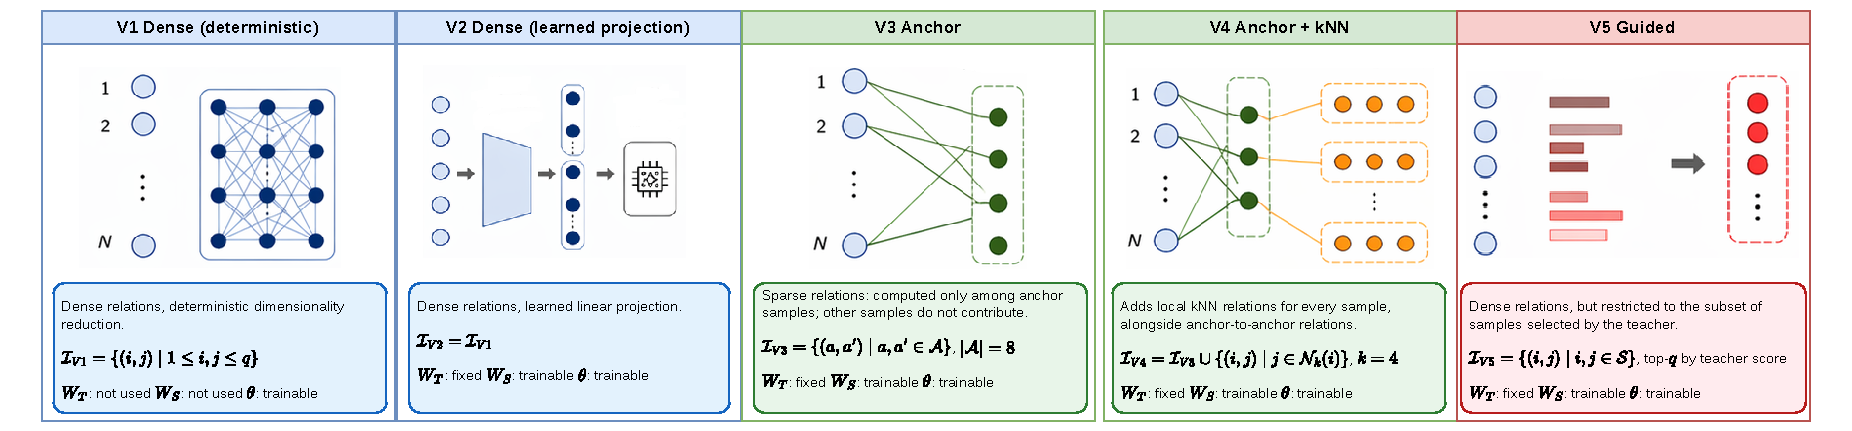
\includegraphics[width=\linewidth]{figs/fig2_QRD.pdf}
\caption{The five variants of the QRD framework.}
\label{fig:bienthe}
\end{figure}
\FloatBarrier

Variants V1 through V4 share one implementation point that needs to
be stated first. Because the cost of simulating the quantum circuit
grows quadratically with the number of samples, the relation matrix
for these four variants is not computed on the entire mini-batch of
size $N$ but on a \emph{position-fixed} subsample. This subsample
consists of the first $q = \min(16, N)$ elements of each batch.
Because the batch has already been shuffled randomly, this subsample
is equivalent to a content-independent random sampling. Every index
set for V1 through V4 below is understood to be defined over those
$q$ samples.

This convention does not apply to V5. In this variant, the
subsample set is determined by a score computed from the entire $N$
samples of the batch rather than from the first $q$ elements. The
difference in candidate pool between V5 and the other four variants
is detailed in the description of V5 below.

\textbf{V1: dense relations, deterministic dimensionality
reduction.} This base variant does not use a learned linear
projection at the dimensionality-reduction step. The quantum circuit
$\theta$ is still trained as in every other variant
(Section~\ref{sec:qrd}), so this variant has 24 additional
parameters (only $\theta$), compared with 604 parameters for the
other four variants (580 from $W_S$ plus 24 from $\theta$). The
$d$-dimensional feature vector is divided evenly into $n_q$
consecutive groups, each averaged:

\begin{equation}
\label{eq:chunk}
\big[g(f)\big]_m = \frac{n_q}{d}
  \sum_{l = (m-1)d/n_q + 1}^{m\,d/n_q} f_l,
  \qquad m = 1,\ldots,n_q,
\end{equation}

and then $g(f)$ replaces $W f$ in \eqref{eq:angles}. The index set
consists of all pairs:

\begin{equation}
\label{eq:i-v1}
\mathcal{I}_{\mathrm{V1}} = \{(i,j) \mid 1 \le i,j \le q\}.
\end{equation}

The index set $\mathcal{I}_{\mathrm{V1}}$ includes the diagonal pairs
$(i,i)$. These elements always have
$R_T^{(Q)}(i,i) = R_S^{(Q)}(i,i) = 1$ by the definition of fidelity,
so they contribute exactly 0 to $\mathcal{L}_{\mathrm{QRD}}$, carry
no information, and generate no gradient. They only slightly dilute
the average in \eqref{eq:qrd} by increasing $|\mathcal{I}|$. This
variant is the most direct extension of classical relational
distillation into Hilbert space and serves as the comparison point
for the other four variants.

\textbf{V2: dense relations, learned projection.} This variant keeps
V1's index set but replaces the deterministic dimensionality
reduction with the two linear projections $W_T$ and $W_S$ described
in Section~\ref{sec:qrd}, in which only $W_S$ is a trainable
parameter while $W_T$ remains fixed:

\begin{equation}
\label{eq:i-v2}
\mathcal{I}_{\mathrm{V2}} = \mathcal{I}_{\mathrm{V1}}.
\end{equation}

The pair V1 and V2 isolates the effect of allowing the model to
learn how to project features into angle space, with every other
factor held fixed.

\textbf{V3: sparse relations based on an anchor set.} To reduce
relation density, this variant restricts the index set to an anchor
set $\mathcal{A}$ of size $M = 8$:

\begin{equation}
\label{eq:i-v3}
\mathcal{I}_{\mathrm{V3}} = \{(a,a') \mid a, a' \in \mathcal{A}\},
\qquad \mathcal{A} \subset \{1,\ldots,q\}, \; |\mathcal{A}| = M.
\end{equation}

The anchor set is taken as the first $M$ elements of the subsample.
The training \texttt{DataLoader} sets \texttt{shuffle=True} and
reshuffles the sample order at every epoch, so this is a random
selection rather than one based on any criterion about sample
content. This choice is deliberate, isolating the effect of
\emph{reducing density} from the effect of \emph{guided selection},
which is investigated in V5. Samples outside $\mathcal{A}$ do not
contribute to the relation loss component, although they still
participate in the other components of \eqref{eq:total}.

\textbf{V4: combining global and local relations.} This variant adds
neighborhood relations to the anchor block:

\begin{equation}
\label{eq:i-v4}
\mathcal{I}_{\mathrm{V4}} = \{(a,a') \mid a,a' \in \mathcal{A}\}
  \cup \{(i,j) \mid j \in \mathcal{N}_k(i)\},
\end{equation}

where $\mathcal{N}_k(i)$ is the set of the $k = 4$ nearest neighbors
of sample $x_i$. Neighbors are determined by Euclidean distance on
the teacher's features, that is, the local structure is taken from
the already-trained model rather than from the student that is still
learning. The resulting relation is symmetrized. If $j$ belongs to
the neighborhood of $i$, both pairs $(i,j)$ and $(j,i)$ belong to
$\mathcal{I}_{\mathrm{V4}}$. Unlike V3, every sample in the subsample
participates through its own neighborhood edges. Because
$\mathcal{I}_{\mathrm{V4}}$ is defined as a set, a pair $(i,j)$ that
appears in both the anchor block and the kNN block is counted
exactly once in \eqref{eq:qrd}, not accumulated. When
\texttt{torch.topk} encounters tied distances among neighbors, the
order returned depends on PyTorch's implementation (stable but with
no statistically meaningful priority). With continuous features as
used here, the probability of an exact distance tie is almost
negligible on real data.

\textbf{V5: teacher-guided relation selection.} The four variants
above select samples independently of content, on a fixed subset of
$q$ elements. V5 replaces that fixed subset with a subset
\emph{selected by content}, with the candidate pool being the entire
$N$ samples of the batch rather than the first $q$ elements. For
each sample $x_i$ in the entire batch ($i = 1,\ldots,N$), the
teacher's uncertainty is measured by the normalized entropy of the
prediction distribution:

\begin{equation}
\label{eq:entropy}
u_i = -\frac{1}{\log C}\sum_{c=1}^{C}
  p_T(c \mid x_i) \log p_T(c \mid x_i),
\end{equation}

where $C$ is the number of classes, so that $u_i \in [0,1]$. The
degree of disagreement between the teacher and the student is
measured by the Jensen--Shannon divergence:

\begin{equation}
\label{eq:js}
d_i = \tfrac{1}{2}\mathrm{KL}\!\left(p_T \,\|\, m_i\right)
    + \tfrac{1}{2}\mathrm{KL}\!\left(p_S \,\|\, m_i\right),
\qquad m_i = \tfrac{1}{2}\left(p_T + p_S\right),
\end{equation}

where $p_T$ and $p_S$ are shorthand for $p_T(\cdot \mid x_i)$ and
$p_S(\cdot \mid x_i)$. Compared with the $L_2$ norm, the
Jensen--Shannon divergence has the advantage of being symmetric,
bounded, and suited to comparing two probability distributions. The
combined score is a weighted average of the two quantities, computed
for all $N$ samples:

\begin{equation}
\label{eq:score}
s_i = w_e\,u_i + w_d\,d_i, \qquad w_e = w_d = 0.5,
\qquad i = 1,\ldots,N.
\end{equation}

The set $\mathcal{S}$ consists of the $q$ samples with the highest
scores selected from the entire $N$ samples. The relation matrix is
constructed on the pairs within that subset of size $q$:

\begin{equation}
\label{eq:i-v5}
\mathcal{I}_{\mathrm{V5}} = \{(i,j) \mid i,j \in \mathcal{S}\},
\qquad \mathcal{S} = \operatorname*{arg\,top\text{-}q}_{i \in \{1,\ldots,N\}} s_i.
\end{equation}

Unlike V1--V4, where the index set $\mathcal{I}$ is determined by a
fixed position or the teacher's frozen features, the selection of
the set $\mathcal{S}$ here depends on the score $s_i$ through a
discrete, non-differentiable selection. Meanwhile, the step of
constructing the relation matrix on $\mathcal{S}$ still requires
normal backpropagation. Algorithm~1 summarizes the computation
sequence and clarifies the gradient boundary between these two
parts.

\begin{quote}
\ttfamily\small
\noindent\textbf{Algorithm 1. Teacher-guided relation selection (V5).}\\[2pt]
\textbf{Input:} teacher logits $Z_T \in \mathbb{R}^{C \times N}$,
student logits $Z_S \in \mathbb{R}^{C \times N}$, teacher/student
features $F_T, F_S \in \mathbb{R}^{d \times N}$, selection set size
$q$.\\
\textbf{Output:} the $q \times q$ quantum relation matrices used for
$\mathcal{L}_{\mathrm{QRD}}$.\\[4pt]
1: \quad \# Steps 1--3 lie outside the gradient graph (torch.no\_grad)\\
2: \quad \textbf{for} $i = 1,\ldots,N$: compute $u_i$ via
\eqref{eq:entropy} from $Z_T$\\
3: \quad \textbf{for} $i = 1,\ldots,N$: compute $d_i$ via
\eqref{eq:js} from $Z_T, Z_S$\\
4: \quad \textbf{for} $i = 1,\ldots,N$: $s_i \leftarrow w_e u_i + w_d d_i$
(\eqref{eq:score})\\
5: \quad $\mathcal{S} \leftarrow$ indices of the $q$ largest values
of $s_i$ among the $N$ samples (\texttt{torch.topk}, no
backpropagation)\\[4pt]
6: \quad \# From here, gradients are reconnected normally\\
7: \quad $F_T[\mathcal{S}],\, F_S[\mathcal{S}] \leftarrow$ extract
the $q$ columns of $F_T, F_S$ at indices $\mathcal{S}$\\
8: \quad Encode $F_T[\mathcal{S}], F_S[\mathcal{S}]$ into quantum
states via \eqref{eq:angles}--\eqref{eq:state}\\
9: \quad Construct $R_T^{(Q)}, R_S^{(Q)} \in \mathbb{R}^{q \times q}$
via \eqref{eq:kernel}--\eqref{eq:relmat} on the $q$ selected samples\\
10: \quad Compute $\mathcal{L}_{\mathrm{QRD}}$ via \eqref{eq:qrd} on
these two $q \times q$ matrices
\end{quote}

Two points should be emphasized to avoid confusion with V1--V4. The
candidate pool for computing the score in lines 2--4 is the entire
$N$ samples of the batch, not the reduced $q$ samples. The
\texttt{top-q} operation in line 5 is therefore a genuine selection
(discarding the $N - q$ lower-scoring samples), unlike V1--V4, which
perform no selection at all once the first $q$ samples have been
fixed by position. In addition, the score $s_i$ is computed from
logits and lies outside the gradient graph (lines 1--5). In
contrast, the quantum relation matrix is still constructed from the
intermediate features $F_T[\mathcal{S}], F_S[\mathcal{S}]$ and fully
participates in backpropagation (lines 6--10). In other words,
output-level information only guides sample selection and does not
replace the features used to measure relations. Because the entropy,
the Jensen--Shannon divergence, and the \texttt{top-}$q$ operation
all lie within \texttt{torch.no\_grad} (lines 1--5), V5's sample
selection is a discrete rule, fixed according to formula
\eqref{eq:score}, rather than a differentiable mechanism optimized
together with the network. Only the step of constructing the
relation matrix on the selected set (lines 6--10) participates in
backpropagation.

Table~\ref{tab:bienthe_cauhinh} summarizes the training status of
each component across all five variants, to avoid confusion between
``no learned projection'' (V1) and ``no trainable parameters at
all'' (which is not true for V1, since the circuit $\theta$ is still
trained). The additional-parameters column does not count the
teacher/student parameters that already exist outside the QRD
branch.

\begin{table}[!htbp]
\centering
\caption{Training status of each component across the five QRD variants.}
\label{tab:bienthe_cauhinh}
\small
\begin{tabular}{lccccc}
\toprule
\textbf{Variant} & $W_T$ & $W_S$ & $\theta$ & Pair set $\mathcal{I}$ & Additional parameters \\
\midrule
V1 Dense (deterministic) & not used & not used & trained & full $q\times q$ & 24 \\
V2 Dense (learned projection) & fixed & trained & trained & full $q\times q$ & 604 \\
V3 Anchor & fixed & trained & trained & anchor $\mathcal{A}$, $M{=}8$ & 604 \\
V4 Anchor$+$kNN & fixed & trained & trained & anchor $+$ kNN, $k{=}4$ & 604 \\
V5 Guided & fixed & trained & trained & teacher top-$q$ & 604 \\
\bottomrule
\end{tabular}
\end{table}
\FloatBarrier

The five variants form two intersecting survey axes. The first axis,
consisting of V1 and V2, examines the adaptability of the
dimensionality reduction. The second axis, consisting of V2 through
V5, examines the density and manner of relation selection, moving
from no intervention, to random density reduction, to adding local
structure, and then to content-based sample selection. In parallel
with these two axes, replacing the quantum kernel function with a
cosine or RBF kernel function within the same strategy isolates the
contribution of the representation space.

\section{Experimental Setup and Results}
\label{sec:thucnghiem}

\subsection{Data, preprocessing, and evaluation protocol}
\label{sec:dulieu}

The method is evaluated on the PhysioNet EEG Motor Movement/Imagery
dataset (referred to as PhysionetMI, after the name of the
corresponding dataset class in MOABB) \cite{schalk2004bci2000,
goldberger2000physiobank}, consisting of EEG recordings from 109
subjects acquired with a 64-electrode system under the 10--10
standard at a sampling frequency of 160 Hz. Six subjects with
recordings inconsistent in duration or label assignment were
excluded according to the exclusion list of the teacher work
\cite{zoumpourlis2024motor}, subject codes 88, 90, 92, 100, 104, and
106. The remaining 103 subjects were used.

The experiments focus on the two-class problem \emph{left\_hand} and
\emph{right\_hand}, following the default two-class paradigm of the
\texttt{PhysionetMI} class in MOABB, distinguishing imagined
left-hand and right-hand grasping, two basic control commands in
brain-signal-operated assistive systems. The three remaining classes
of the original dataset (rest, feet, hands) were not used. The
number of trials per subject is not fixed, varying according to the
actual number of recordings retained. No additional class-balancing
step was applied beyond the original paradigm.

The raw signal sampled at 160 Hz is processed through four
sequential steps: 4--38 Hz bandpass filtering (a zero-phase FIR
filter under the default MNE/braindecode configuration, without
explicit order tuning); Common Average Reference re-referencing;
resampling to 100 Hz; and windowing. There is no notch filtering
step, no explicit artifact-removal step (no ICA, no trial-rejection
threshold), and no normalization other than converting units from
volts to microvolts. Therefore, no data-leakage risk arises from
fitting a normalization on the whole dataset. Each epoch begins
exactly at the event onset, with no start or end offset delay, and
lasts 3.0 s, corresponding to 300 samples at 100 Hz after resampling.

The evaluation protocol is 5-fold cross-validation split by subject,
to ensure that no subject appears simultaneously in the training set
and the test set. This setup reflects real deployment conditions,
where the system must operate with users who never participated in
training.

Folds are split according to a deterministic rule. All 103 valid
subjects, keeping their code order, are divided into 5 consecutive,
nearly equal blocks. For each fold index, one block is chosen as the
test set, the next block in cyclic order as the validation set, and
the remaining three blocks as the training set. The corresponding
proportions are approximately 62 for training, 21 for validation,
and 20 for testing. The validation set is always completely
separated by subject from both other sets. This split does not
depend on the random seed. The same fold index always yields the
same set of subjects across all five seeds. The seed governs only
the randomness of training (weight initialization, batch order), not
how the data is split. The complete list of 515 subject-to-fold
assignments is provided with the published source code but is not
printed in the paper because of its length.

The entire procedure is repeated with five independent random seeds.
The statistical unit used to compute the accuracy score of each
configuration is the subject, not the trial or the fold, in order to
avoid overly optimistic evaluation caused by the high correlation
among samples within the same subject. Each subject enters the test
set exactly once across the 5 folds, so each configuration is
aggregated over $5 \times 103 = 515$ per-subject results.

\subsection{Teacher and student network architectures}
\label{sec:kientruc}

The teacher--student pair was chosen to maximize the separation
between representational capacity and deployability. The teacher is
Ensemble-MI \cite{zoumpourlis2024motor}, a classification system
consisting of multiple convolutional branches operating in parallel.
It is trained using a curriculum and collaborative learning
mechanism. With about 15.1 thousand parameters, this model is about
6.3 times larger than the student and 7.1 times slower in inference
time, because computational cost scales with the number of branches.
The teacher is trained separately for each fold, yielding 5
independent checkpoints corresponding exactly to the 5 data splits
in Section~\ref{sec:dulieu}. Each checkpoint is trained for 120
epochs with 7 collaborative-learning subsets, following the original
Ensemble-MI procedure exactly.

The student is EEGNet \cite{lawhern2018eegnet}, using depthwise and
separable convolutions to sharply reduce the number of parameters.
With about 2.4 thousand parameters (2,402, about 10.2 million MACs
per inference, see Section~\ref{sec:ketqua}), this architecture has
the potential to be deployed on a microcontroller. This parameter
scale is in the same class as a published EEGNet deployment on
embedded hardware \cite{wang2024mibminet}, although it has not been
directly verified on that exact class of ultra-low-power
microcontroller. Section~\ref{sec:danhgiadk} reports a direct
inference-time measurement on real embedded hardware (Raspberry Pi
4). Both models produce intermediate feature vectors of the same
dimensionality $d = 144$, so the feature-level and relation-level
loss functions are applied directly without an intermediate
projection layer.

The teacher is pretrained, kept fixed, and has gradient updates
disabled throughout the entire distillation process. On this
dataset, the teacher achieves an accuracy of $84.98\% \pm 2.59\%$
(mean and standard deviation over 5 folds).

\subsection{Experimental configuration and hyperparameters}
\label{sec:cauhinh}

All experiments are implemented using PyTorch combined with
PennyLane, running on a single GPU of a high-performance computing
system. Table~\ref{tab:cauhinh} summarizes the full configuration.

\begin{table}[!htbp]
\centering
\caption{Experimental configuration and hyperparameters.}
\label{tab:cauhinh}
\small
\begin{tabular}{@{}ll@{\hspace{2.2em}}ll@{}}
\toprule
\multicolumn{2}{@{}l}{\textit{Data and protocol}}
  & \multicolumn{2}{l@{}}{\textit{Loss weights}} \\
\cmidrule(r){1-2}\cmidrule(l){3-4}
Dataset & PhysionetMI          & $\alpha$ (cross-entropy) & 0.5 \\
Number of subjects & 103 out of 109        & $\tau$ (temperature)      & 4.0 \\
Channels, sampling rate & 64, 160 Hz          & $\gamma_f$ (FeatureKD) & 1.0 \\
Task & Two-class                 & $\gamma_r$ (RelationalKD) & 1.0 \\
Cross-validation & 5-fold by subject  & $\beta$ (QRD)          & 0.02 \\
Number of seeds & 5                   & & \\
Statistical unit & Subject        & \multicolumn{2}{l@{}}{\textit{Quantum and relation selection}} \\
\cmidrule(r){1-2}\cmidrule(l){3-4}
\multicolumn{2}{@{}l}{\textit{Model}}
  & Number of qubits $n_q$ & 4 \\
\cmidrule(r){1-2}
Teacher & Ensemble-MI, $15.1$ K  & Number of entangling layers $L$ & 2 \\
Student & EEGNet, $2.4$ K        & Circuit weights & trainable \\
Feature dimension $d$ & 144          & Subsample size $q$ & 16 \\
 & & Number of anchor samples $M$ & 8 \\
\multicolumn{2}{@{}l}{\textit{Optimization}}
  & Number of neighbors $k$ & 4 \\
\cmidrule(r){1-2}
Optimizer & SGD, momentum 0.9      & $w_e$, $w_d$ & 0.5 and 0.5 \\
Learning rate & 0.005              & & \\
Weight decay & 0.01                & & \\
Batch size & 64                    & & \\
Number of epochs & 30                      & & \\
Checkpoint selection & by validation accuracy & & \\
Library & PyTorch, PennyLane      & & \\
\bottomrule
\end{tabular}
\end{table}
\FloatBarrier

Every distillation configuration shares the same teacher, student,
dataset, fold split, seed set, and all optimization hyperparameters.
The only component that changes across configurations is the
knowledge-transfer mechanism. Because of this constraint, any
observed performance difference cannot be attributed to differences
in architecture or training procedure.

The coefficient $\alpha$ in Table~\ref{tab:cauhinh} specifically
applies to configurations with a distillation term, where it
balances the cross-entropy against the distillation loss. The
no-distillation configuration has no second term to balance against,
so it uses $\alpha = 1.0$ (full cross-entropy) instead of $0.5$,
following the same full-weight principle applied to every other
configuration in Table~\ref{tab:cauhinh}. Every ``no-distillation''
figure in the paper from this point onward uses $\alpha = 1.0$.

Both this choice of $\alpha = 1.0$ and the choice of $\beta = 0.02$
(reasoning given in Section~\ref{sec:qrd}) are checked for
sensitivity by training further at other values:
$\alpha \in \{0; 0.25; 0.5; 0.75\}$ for the no-distillation
configuration, and $\beta \in \{0.01; 0.05\}$ for V5 Guided
specifically (the quantum kernel function, the main representative
configuration for the quantum branch in Section~\ref{sec:danhgiadk}).
These two $\beta$ values are, respectively, half of and 2.5 times
the nominal level. The $\beta$ control does not extend to cosine or
RBF. The results of the $\alpha$ sensitivity are presented in
Section~\ref{sec:hieuqua}, and the results of the $\beta$ sensitivity
in Section~\ref{sec:chuyensau}.

\subsection{Results and discussion}
\label{sec:ketqua}

Before presenting the results, the statistical unit used for the
tests below needs to be clarified. Each configuration is aggregated
over 515 per-subject results (Section~\ref{sec:dulieu}). These
results are not independent of one another. Subjects within the same
fold of the same seed share a single trained student model. For this
reason, the unit of inference for the hypothesis tests in this part
is the seed, not the subject. Each seed reduces the 515 results
above to a single mean value. Every paired $t$-test in the paper
therefore uses $n = 5$ independent pairs, with $df = 4$ degrees of
freedom. The ``mean $\pm$ standard deviation'' values reported in
the tables below are likewise computed over exactly these five
per-seed values, not over the 515 per-subject results.

This choice of inference unit has a limitation worth noting. It
confirms whether the conclusion is robust to the randomization of
training. But it does not confirm whether the conclusion generalizes
to a different subject population, because every seed is evaluated
on exactly the same set of 103 subjects. The generalization question
is addressed separately through replication on Cho2017 (presented
below), which is exploratory rather than confirmatory. The kernel
comparison specifically also uses an additional subject-by-seed
cross analysis in Section~\ref{sec:chuyensau}.

\subsubsection{Distillation effect and the degree of separation among mechanisms}
\label{sec:hieuqua}

This part presents evidence for the effectiveness and stability of
knowledge distillation, first on PhysionetMI, then checked against a
second independent motor imagery dataset.

\begin{table}[!htbp]
\centering
\caption{Comparison of distillation mechanisms on PhysionetMI.}
\label{tab:tongthe}
\begin{tabular}{lccc}
\toprule
\textbf{Configuration} & \textbf{Accuracy (\%)} & $\boldsymbol{\Delta}$ & $\boldsymbol{p}$ \\
\midrule
No distillation (student alone) & $74.93 \pm 2.30$ & $-6.56$ & $0.002$ \\
\textbf{Logit distillation (KDBase)} & $81.49 \pm 0.59$ & -- & -- \\
Feature distillation (FeatureKD) & $80.05 \pm 1.02$ & $-1.44$ & $0.016$ \\
Euclidean relational distillation (RelationalKD) & $81.61 \pm 0.84$ & $+0.12$ & $0.754$ \\
V1 Dense & $81.90 \pm 0.71$ & $+0.41$ & $0.158$ \\
V2 Dense & $81.49 \pm 0.78$ & $+0.00$ & $1.000$ \\
V3 Anchor & $81.25 \pm 1.00$ & $-0.24$ & $0.351$ \\
V4 Anchor $+$ kNN & $81.42 \pm 0.75$ & $-0.07$ & $0.775$ \\
V5 Guided & $81.12 \pm 0.71$ & $-0.37$ & $0.231$ \\
\bottomrule
\end{tabular}
\end{table}
\FloatBarrier

Table~\ref{tab:tongthe} presents the results of the distillation
mechanisms. The $\Delta$ column is the difference relative to
KDBase (the reference row, $\Delta=0$), and the $p$ column is the
paired $t$-test over seeds. The largest and clearest effect lies in
whether distillation is present or not. The independently trained
student reaches 74.93\%, while every distillation configuration
reaches about 81\%. The improvement from adding distillation is 6.56
percentage points (95\% confidence interval from 4.08 to 9.04
points, $p = 0.0018$), computed in the direction opposite to the
table's $\Delta$ column, which subtracts using KDBase as the
reference. This is an effect that far exceeds every other source of
variation in the experiment.

This result raises the question of whether the 6.56-percentage-point
improvement depends on the specific choice of $\alpha = 1.0$ for the
no-distillation configuration. To check this, the no-distillation
configuration was trained further at four other values of $\alpha$.

Table~\ref{tab:alphasweep} shows that accuracy increases
monotonically with $\alpha$, from near-chance level ($\alpha=0$, no
supervisory signal from the true labels at all) to $74.93\%$ at
$\alpha=1.0$. If the distillation improvement
is computed at $\alpha = 0.5$ instead of $\alpha = 1.0$, the
independent student reaches only $63.06\%$, pushing the observed
improvement up to $18.43$ percentage points, nearly three times the
$6.56$-point figure above. The difference between the two ways of
computing this does not reflect two comparable estimates of the same
effect; rather, it reflects that $\alpha = 0.5$ does not give the
no-distillation configuration enough weight on the one loss term it
has. $\alpha = 1.0$ is the value consistent with the full-weight
principle applied to every other configuration in the paper.

\begin{table}[!htbp]
\centering
\caption{Sensitivity of the no-distillation configuration to the
coefficient $\alpha$ (PhysionetMI, 5 seeds $\times$ 5 folds).}
\label{tab:alphasweep}
\begin{tabular}{cc}
\toprule
$\boldsymbol{\alpha}$ & \textbf{Accuracy (\%)} \\
\midrule
0.00 & $49.89 \pm 0.34$ \\
0.25 & $51.73 \pm 2.68$ \\
0.50 & $63.06 \pm 5.03$ \\
0.75 & $71.45 \pm 3.74$ \\
1.00 (used for the main baseline) & $\boldsymbol{74.93 \pm 2.30}$ \\
\bottomrule
\end{tabular}
\end{table}
\FloatBarrier

Distillation narrows most, but not all, of the gap to the teacher
(which reaches $84.98\%$). With the reference configuration KDBase,
the remaining gap is 3.49 percentage points, compared with the
10.05-percentage-point gap of the non-distilled student. This
narrowing corresponds to about 65\% of the initial capability gap
between the two models.

The FeatureKD configuration reaches 80.05\%, 1.44 points lower than
KDBase, with $p = 0.016$. This result has two implications. On one
hand, the constraint of directly aligning features by squared error
appears too rigid for EEG signals, forcing the student to reproduce
representational components that are irrelevant to the
classification task. On the other hand, the protocol did detect this
1.44-percentage-point effect in that specific comparison. A
comparison reaching significance does not automatically guarantee
equivalent power for every other comparison, because power depends
on the variance specific to each pair. With the observed standard
deviation of the paired difference in this comparison (0.80
percentage points, $n=5$), the minimum detectable effect at 80\%
power is about 1.33 percentage points. This figure is only slightly
below the observed 1.44 points, showing that this is a
near-boundary detection rather than one with a large power margin.

Against this backdrop, the results of the relation-based mechanisms
become noteworthy. RelationalKD (Euclidean, classical) reaches
81.61\%, 0.12 points higher than KDBase ($p = 0.754$). The five QRD
variants (quantum kernel function, V1--V5) range from 81.12\% (V5
Guided) to 81.90\% (V1 Dense). No variant separates from KDBase at a
statistically significant level; the smallest $p$ is $0.158$ (V1
Dense). Placed side by side, these two figures clearly show the
focus of the paper's contribution. Knowledge distillation in general
provides 6.56 percentage points (74.93\%~$\to$~81.49\%), whereas all
five QRD variants together with RelationalKD span only a range of
0.78 percentage points (81.12\%~$\to$~81.90\%) around that mark.
Section~\ref{sec:chuyensau} analyzes in detail each design axis that
produces the variation observed above.

\paragraph{Replication on a second independent dataset (Cho2017)}

This part reports an additional, exploratory survey on a second
motor imagery dataset, to qualitatively check the generality of the
conclusions from the parts above. No hypothesis or equivalence
margin was specified before running, so the results below are used
only for qualitative comparison with the conclusions on PhysionetMI
and do not replace the main comparison in that part.

The Cho2017 dataset \cite{cho2017eeg}, accessed via the
\texttt{Cho2017} class in MOABB, consists of 52 subjects performing
imagined left-hand and right-hand grasping. Three subjects (32, 46,
49) were excluded according to the default list used for the teacher
\cite{zoumpourlis2024motor}, leaving 49 subjects used, with the same
two-class task as PhysionetMI. The training protocol, teacher/student
architecture, and all hyperparameters remain the same as in
Section~\ref{sec:cauhinh}. Only the fold-splitting protocol changes
with the number of subjects, using 5 nearly equal blocks over 49
subjects instead of 103. The teacher achieves an accuracy of
$75.07\% \pm 4.16\%$ (mean and standard deviation over 5 folds),
lower and more variable than on PhysionetMI ($84.98\% \pm 2.59\%$).

The seven configurations using the quantum kernel function on
Cho2017 (V1 Dense, V2 Dense, V3 Anchor, V4 Anchor+kNN, V5 Guided, and
the two $\beta$ variants of V5) were trained with the quantum
circuit described in Section~\ref{sec:qrd}. The six classical
configurations that do not use the quantum kernel function (No KD,
KDBase, FeatureKD, RelationalKD, cosine kernel, RBF kernel) do not
depend on the quantum circuit and therefore keep their existing
figures. Table~\ref{tab:cho2017} reports the resulting accuracy for
all twelve configurations.

\begin{table}[!htbp]
\centering
\caption{Results on Cho2017 (49 subjects, 5 independent seeds).}
\label{tab:cho2017}
\begin{tabular}{lccc}
\toprule
\textbf{Configuration} & \textbf{Accuracy (\%)} & $\boldsymbol{\Delta}$ & $\boldsymbol{p}$ \\
\midrule
No KD & $70.32 \pm 0.64$ & $-2.22$ & 0.0018 \\
KDBase & $72.54 \pm 0.21$ & --- & --- \\
FeatureKD & $71.17 \pm 0.69$ & $-1.38$ & 0.003 \\
RelationalKD & $72.57 \pm 0.42$ & $+0.03$ & 0.864 \\
\midrule
V1 Dense & $72.31 \pm 0.69$ & $-0.24$ & 0.405 \\
V2 Dense & $72.37 \pm 0.43$ & $-0.18$ & 0.343 \\
V3 Anchor & $72.03 \pm 0.63$ & $-0.51$ & 0.110 \\
V4 Anchor $+$ kNN & $72.28 \pm 0.56$ & $-0.26$ & 0.182 \\
V5 Guided & $72.41 \pm 0.65$ & $-0.13$ & 0.626 \\
V5 Guided ($\beta = 0.01$) & $72.17 \pm 0.38$ & $-0.37$ & 0.018 \\
V5 Guided ($\beta = 0.05$) & $72.36 \pm 0.27$ & $-0.19$ & 0.091 \\
\midrule
Cosine kernel & $72.13 \pm 0.30$ & $-0.41$ & 0.030 \\
RBF kernel & $72.36 \pm 0.52$ & $-0.18$ & 0.452 \\
\bottomrule
\end{tabular}
\end{table}
\FloatBarrier

Table~\ref{tab:sosanh2dataset} places $\Delta$ relative to KDBase
side by side between PhysionetMI (the main comparison) and Cho2017
(the exploratory survey) for each configuration. The last column
marks Yes if the sign direction agrees between the two datasets,
regardless of whether statistical significance is reached. The
\emph{No KD} row records the 95\% confidence interval instead of
$p$, following the same way this effect was reported above. Three
qualitative findings from the parts above are discussed in detail
below the table.

Six of the twelve rows in Table~\ref{tab:sosanh2dataset} change sign
direction between the two datasets: V1 Dense, V2 Dense, the cosine
kernel, the RBF kernel, and both direct kernel comparisons. In all
six cases, $\Delta$ on at least one of the two datasets is smaller
than $0.5$ percentage points, that is, it lies in a region near
$\Delta = 0$ where the sign can easily flip from seed noise alone.
The cosine kernel row specifically has $p = 0.030$ on Cho2017,
discussed separately below. The remaining five cases do not reach
statistical significance on either dataset.

The distillation effect replicates on Cho2017. No KD ($\alpha = 1.0$,
the same full-weight principle applied on PhysionetMI,
Section~\ref{sec:cauhinh}) reaches $70.32\%$ versus $72.54\%$ for
KDBase, a difference of $2.22$ percentage points (95\% confidence
interval $[1.39, 3.06]$, $p = 0.0018$). The direction and
significance of the effect remain the same as on PhysionetMI, but
the magnitude is considerably smaller: $2.22$ points on Cho2017
versus the $6.56$ points on PhysionetMI noted above, less than half.
Part of the difference may come from the smaller teacher-student
capacity gap on Cho2017. The teacher-minus-non-distilled-student gap
is $4.75$ percentage points on Cho2017 ($75.07\%$ minus $70.32\%$),
compared with $10.05$ points on PhysionetMI, leaving less room for
distillation to narrow.

\begin{table}[!htbp]
\centering
\caption{Side-by-side comparison of $\Delta$ relative to KDBase
between PhysionetMI and Cho2017 for each configuration.}
\label{tab:sosanh2dataset}
\small
\begin{tabular}{lccc}
\toprule
\textbf{Configuration} & \textbf{PhysionetMI} & \textbf{Cho2017} & \textbf{Same direction} \\
\midrule
No KD & $-6.56$ (CI95\% $[4.08;9.04]$) & $-2.22$ (CI95\% $[1.39;3.06]$) & Yes \\
FeatureKD & $-1.44$ ($p=0.016$) & $-1.38$ ($p=0.003$) & Yes \\
RelationalKD & $+0.12$ ($p=0.754$) & $+0.03$ ($p=0.864$) & Yes \\
V1 Dense & $+0.41$ ($p=0.158$) & $-0.24$ ($p=0.405$) & No \\
V2 Dense & $+0.00$ ($p=1.000$) & $-0.18$ ($p=0.343$) & No \\
V3 Anchor & $-0.24$ ($p=0.351$) & $-0.51$ ($p=0.110$) & Yes \\
V4 Anchor $+$ kNN & $-0.07$ ($p=0.775$) & $-0.26$ ($p=0.182$) & Yes \\
V5 Guided & $-0.37$ ($p=0.231$) & $-0.13$ ($p=0.626$) & Yes \\
Cosine kernel & $+0.14$ ($p=0.609$) & $-0.41$ ($p=0.030$) & No \\
RBF kernel & $+0.13$ ($p=0.511$) & $-0.18$ ($p=0.452$) & No \\
\midrule
\multicolumn{4}{l}{\textit{Direct kernel comparison within the same V5 strategy (not versus KDBase)}} \\
Quantum versus cosine & $-0.51$ ($p=0.096$) & $+0.28$ ($p=0.389$) & No \\
Quantum versus RBF & $-0.49$ ($p=0.060$) & $+0.05$ ($p=0.903$) & No \\
\bottomrule
\end{tabular}
\end{table}
\FloatBarrier

The difference among distillation mechanisms remains smaller than
seed noise, although the safety margin is thinner. The standard
deviation across the twelve mechanisms (excluding No KD) is $0.37$
percentage points. The average standard deviation from seeds is
$0.48$ points. The ratio between the two quantities is $0.77$. On
PhysionetMI, the corresponding ratio is $0.61$. The qualitative
conclusion holds, but the gap between the two sources of variation
is narrower.

Two other specific findings also replicate almost exactly. FeatureKD
is $1.38$ points worse than KDBase ($p = 0.003$), versus $1.44$
points ($p = 0.016$) on PhysionetMI. Classical RelationalKD does not
differ from KDBase, a difference of $0.03$ points ($p = 0.864$)
versus $0.12$ points ($p = 0.754$) on PhysionetMI.

The main kernel comparison, between the quantum kernel function and
the cosine kernel function within the same V5 strategy, changes sign
direction between the two datasets. On PhysionetMI, the quantum
kernel function is $0.51$ points lower than cosine. On Cho2017, the
quantum kernel function is $0.28$ points higher than cosine (95\%
confidence interval $[-0.52, 1.08]$, $p = 0.389$). Both confidence
intervals are wide and cover zero. This change in direction does not
contradict the main conclusion already reported; rather, it
reinforces the assessment that there is not yet consistent evidence
for a systematic difference between the two kernel types.

Two results in Table~\ref{tab:cho2017} have no corresponding direct
comparison on PhysionetMI and are therefore only reported rather
than interpreted beyond what the data allows. The cosine kernel is
$0.41$ points lower than KDBase, with $p = 0.030$, on Cho2017. The
main results table on PhysionetMI only compares the kernel functions
with one another and does not directly compare cosine with KDBase,
so there is no basis for calling this a ``non-replicating'' result.
Similarly, V5 Guided ($\beta = 0.01$) is $0.37$ points lower than
KDBase, with $p = 0.018$, on Cho2017.

Overall, the exploratory survey on Cho2017 finds nothing that
contradicts the paper's two main conclusions. Knowledge distillation
provides a large and stable benefit. The difference among specific
knowledge-transfer mechanisms, including the choice of kernel
function, lies below or around the detection threshold of the
5-seed design. This is an exploratory result on a supplementary
dataset and does not replace the main comparison on PhysionetMI.

\subsubsection{In-depth analysis of variant behavior}
\label{sec:chuyensau}

This part analyzes in depth the behavior of the twelve distillation
mechanisms within the design space of the QRD framework. First, each
design axis, the relation-formation strategy and the kernel function
type, is isolated separately to see which axis produces differences
among configurations. This part also includes controls that check
the sensitivity of that conclusion, and a qualitative illustration
using t-SNE. Two other design assumptions noted in
Section~\ref{sec:qrd}, the mechanism of sharing the circuit
parameters $\theta$ and the way $W_T$ is initialized, are examined
afterward and close out this part. The following
Section~\ref{sec:xephang} separately quantifies the noise from
random seeds and the stability of the method ranking across repeated
runs.

\paragraph{Relation-formation strategy and kernel function type}

Table~\ref{tab:bienthe} is divided into three blocks to isolate
three design questions.

\begin{table}[!htbp]
\centering
\caption{Comparison of five relation-formation strategies and two
classical kernel function controls.}
\label{tab:bienthe}
\begin{tabular}{lccc}
\toprule
\textbf{Configuration} & \textbf{Accuracy (\%)} & $\boldsymbol{\Delta}$ & $\boldsymbol{p}$ \\
\midrule
\multicolumn{4}{l}{\textit{Quantum kernel, varying the dimensionality reduction}} \\
V1 Dense, deterministic dimensionality reduction & $81.90 \pm 0.71$ & $+0.41$ & $0.158$ \\
V2 Dense, learned projection & $81.49 \pm 0.78$ & $+0.00$ & $1.000$ \\
\midrule
\multicolumn{4}{l}{\textit{Quantum kernel, varying the relation strategy}} \\
V3 Anchor & $81.25 \pm 1.00$ & $-0.24$ & $0.351$ \\
V4 Anchor $+$ kNN & $81.42 \pm 0.75$ & $-0.07$ & $0.775$ \\
V5 Guided & $81.12 \pm 0.71$ & $-0.37$ & $0.231$ \\
\midrule
\multicolumn{4}{l}{\textit{Fixed V5 strategy, varying the kernel function}} \\
Cosine kernel & $81.63 \pm 0.63$ & $+0.14$ & $0.609$ \\
RBF kernel & $81.61 \pm 0.58$ & $+0.13$ & $0.511$ \\
Quantum kernel & $81.12 \pm 0.71$ & $-0.37$ & $0.231$ \\
\bottomrule
\end{tabular}
\end{table}
\FloatBarrier

In the first block, the relation set is fixed and the
dimensionality reduction is varied to answer the question of
whether the adaptability of the dimensionality reduction makes a
difference. Variant V1 uses a deterministic, parameter-free
projection, while V2 replaces it with a learned linear projection on
the student side ($W_S$, 580 parameters). The teacher-side projection
$W_T$ remains fixed in both variants (see
Table~\ref{tab:bienthe_cauhinh}). V1 reaches $81.90\%$, $0.41$
percentage points higher than V2 in the direct V1-versus-V2
comparison ($p = 0.085$, distinct from the $p$ column in
Table~\ref{tab:bienthe}, which compares each variant individually
against KDBase). This difference lies in a borderline region, not
reaching the conventional $\alpha = 0.05$ threshold but running
counter to the design expectation. The learned linear projection
shows no measurable benefit over a parameter-free deterministic
dimensionality reduction. The available data even suggests the
opposite direction. The adaptability of the dimensionality
reduction, in this setup, contributes no measurable benefit to the
quality of the relational supervisory signal.

In the second block, the dimensionality reduction is fixed and the
relation-selection strategy is varied to answer the question of
whether the way the relation set is determined makes a difference.
The three variants yield results from 81.12\% to 81.42\%, spanning a
range of 0.30 percentage points. No variant separates from KDBase,
with the smallest $p$ value being 0.231. The observed ordering also
does not match the prediction from the design rationale. The V5
strategy, which was expected to select the most informative
relations, in fact gives the lowest result in the group.

V5 differs from V2--V4 along two dimensions at once: not only the
selection criterion, but also the candidate pool (the entire 64
samples of the batch, versus the 16 position-fixed samples, as noted
above). V5's low result could therefore come from the selection
criterion, from the larger candidate pool, or from both. To separate
these two factors, an additional control variant
(\emph{random\_pool64}) was trained, keeping V5's 64-sample candidate
pool but selecting randomly instead of by the entropy-and-disagreement
criterion. The measured result ($81.36\%$) does not differ
significantly from either V2 or V5, so the available data does not
rule out either of the two factors above.

In the third block, the V5 strategy is fixed and the kernel function
type is varied to answer the central question of the paper: whether
the quantum kernel function separates from the two classical kernel
functions. The three kernel function types span a wider range, 0.51
percentage points: cosine 81.63\%, RBF 81.61\%, and quantum 81.12\%.
The comparison among kernel functions is carried out within the same
V5 strategy, because V5 keeps the relation-selection mechanism
(teacher-guided) and every other hyperparameter fixed, allowing the
effect of the kernel function alone to be isolated from the effect
of the relation-selection strategy.

Does the conclusion above hold up when the crossed structure between
subject and seed is properly handled? All 103 subjects within each
seed share a single trained model, while the five seeds are
evaluated on exactly the same set of subjects, exactly as noted in
the limitation on the inference unit above. Both of these dependency
dimensions need to be handled simultaneously. For the kernel
comparison specifically, a mixed-effects regression model with
crossed random effects for both subject and seed (maximum-likelihood
estimation) is used as an additional analysis that directly handles
that structure, cross-checked with a subject-clustered bootstrap
(10,000 iterations) to avoid depending on distributional
assumptions. Both approaches give the same range of results. The
cosine-minus-quantum difference is $0.50$ percentage points (95\%
confidence interval $[0.00, 1.01]$, $p \approx 0.05$). The
RBF-minus-quantum difference is $0.49$ percentage points (95\%
confidence interval $[-0.01, 0.99]$, $p \approx 0.05$-$0.06$). The
paired $t$-test over the five seeds, following the protocol fixed
before running, gives $p = 0.096$ (cosine) and $p = 0.060$ (RBF),
neither reaching the significance threshold. This preregistered
protocol is reported in parallel for transparency. The result of
this protocol is not superseded by the additional analyses above.

Two points make the results above insufficient to reverse the
conclusion. These are two comparisons within the same comparison
family, cosine and RBF both against quantum. A minimal Bonferroni
correction for two comparisons brings the significance threshold to
$0.025$, which none of the $p$ values above reach. The observed
effect size, about $0.49$-$0.50$ percentage points, nearly coincides
with the pre-specified equivalence margin of $\pm 0.5$ percentage
points, the threshold the paper set for itself as the smallest
difference still practically meaningful for control-channel
bandwidth. Even if measured with higher power, any effect present
would lie right at the boundary of practical unimportance, not a
large effect missed for lack of power. The correct conclusion, using
both analyses, remains \emph{not enough data to draw a definitive
conclusion in either direction}, rather than either equivalence or a
significant difference. Between the two classical kernel functions
themselves, cosine and RBF do not differ ($p = 0.920$, the original
test over seeds).

This is precisely the case that Section~\ref{sec:qrd} anticipated.
If even the relation description by the quantum kernel function does
not separate from the baseline, or if the data obtained are not
sufficient to conclude in any direction, the statement about the
role of relation structure in distillation would have a considerably
broader scope, \emph{with respect to the choice of representation
space}. Broader scope here means that the statement holds not only
for classical metric spaces, but also for a space that is
fundamentally different in nature. Neither case is equivalent to
confirming that the representation space plays no role at all. That
would be a stronger claim than the available data allows.

This reasoning does not extend the scope of the conclusion to other
datasets or problems. The entire survey remains limited to
PhysionetMI and the two-class discrimination problem, described in
Section~\ref{sec:dulieu}.

The conclusion above raises two further questions. The first
question: is the gap between the quantum kernel function and the two
classical kernel functions due to a non-equivalent input space, the
raw 144-dimensional features for cosine and RBF versus the space
learned through $W_S$ for the quantum kernel function? To check
this, cosine and RBF were recomputed on features projected through
the learned $W_S$ and the fixed $W_T$ (580 parameters), identical to
the quantum branch, instead of on the raw features. The result is
projected cosine $81.25\pm0.70\%$ and projected RBF $81.36\pm0.91\%$.
Neither differs significantly from the original 144-dimensional
version (cosine $\Delta=-0.38$pp, $p=0.168$; RBF $\Delta=-0.25$pp,
$p=0.293$), nor differs significantly from quantum V5 (projected
cosine $\Delta=+0.13$pp, $p=0.647$; projected RBF $\Delta=+0.24$pp,
$p=0.312$; $n=5$, $df=4$ for every comparison). The gap between
quantum and the two classical kernel functions narrows relative to
the raw features (down to $0.13$-$0.24$ points, versus $0.49$-$0.51$
points when compared on the raw features), rather than widening.

The second question: does the conclusion depend on the specific
choice of $\beta = 0.02$, and is using a shared $\beta$ across all
three kernel function types actually fair, or does it inadvertently
give one kernel function far more influence than the other two? To
answer the first part, the V5 Guided variant was trained further at
$\beta = 0.01$ and $\beta = 0.05$, one value half of and one value
2.5 times the nominal level (the reason for choosing $\beta = 0.02$
was given in Section~\ref{sec:qrd}). Neither of these two variants
separates from KDBase at a statistically significant level:
$\beta = 0.01$ reaches $81.47\%$ ($\Delta = -0.02$ percentage
points, $p = 0.91$), $\beta = 0.05$ reaches $81.42\%$ ($\Delta =
-0.07$ percentage points, $p = 0.82$), compared with $81.12\%$
($\Delta = -0.37$ percentage points, $p = 0.23$) at the nominal
level. Both alternative values also do not differ significantly
from the nominal level itself ($p = 0.15$ and $p = 0.40$).

To answer the second part, an additional diagnostic (gradNormS)
directly measures the raw value of $\mathcal{L}_{\mathrm{QRD}}$
before multiplying by $\beta$, and the $L_2$ norm of the gradient
that $\beta\,\mathcal{L}_{\mathrm{QRD}}$ alone induces on the
student's parameters, limited to 1 fold and the first 5 epochs on
PhysionetMI. The diagnostic uses the V5 Guided configuration for
cosine and RBF, while the quantum kernel function uses V2 Dense (the
same \texttt{dense} strategy, differing from V5 only in the index
set, which does not affect the quantity measured here), measured
independently with a separate backpropagation pass on the first
batch of each epoch.

\begin{table}[!htbp]
\centering
\caption{Diagnostic of the effective supervisory magnitude of
$\mathcal{L}_{\mathrm{QRD}}$ by kernel function type, at the shared
nominal $\beta = 0.02$.}
\label{tab:betafair}
\begin{tabular}{lccc}
\toprule
\textbf{Kernel} & \textbf{Raw} $\mathcal{L}_{\mathrm{QRD}}$ & $\|\nabla_{\mathrm{student}}\|_2$ & \textbf{Multiple (vs.\ cosine)} \\
\midrule
Cosine  & $2.16 \times 10^{-3}$ & $7.54 \times 10^{-5}$ & $1\times$ \\
RBF     & $3.13 \times 10^{-2}$ & $1.47 \times 10^{-3}$ & $\approx 20\times$ \\
Quantum & $1.41 \times 10^{-1}$ & $1.51 \times 10^{-2}$ & $\approx 200\times$ \\
\bottomrule
\end{tabular}
\end{table}
\FloatBarrier

Table~\ref{tab:betafair} shows that the same nominal $\beta$
produces an effective supervisory magnitude differing by up to two
orders of magnitude between the quantum kernel function and cosine.
RBF is closer to the quantum scale than to cosine, consistent with
how the two kernels self-normalize (RBF by the median distance of
each batch, whereas the quantum kernel function tends to concentrate
values near the boundary because of the geometry of Hilbert space).
Because these are diagnostic figures from one fold and the first
five epochs without repetition over seeds, the specific numbers
should not be regarded as accurate to the last digit, but the
magnitude of the difference (tens to hundreds of times) is clear
enough to rule out the possibility that the three kernel functions
receive an equivalent level of supervision when sharing
$\beta = 0.02$. This is a limitation that has been directly measured
with data, noted again in Section~\ref{sec:ketluan}.

None of the controls above changes the main conclusion of this part.
No relation variant or kernel function separates from KDBase,
whether by controlling the input space more tightly, changing the
value of $\beta$, or accounting for the non-uniform effective
supervision level among the kernel functions.

\begin{figure}[!htb]
\centering
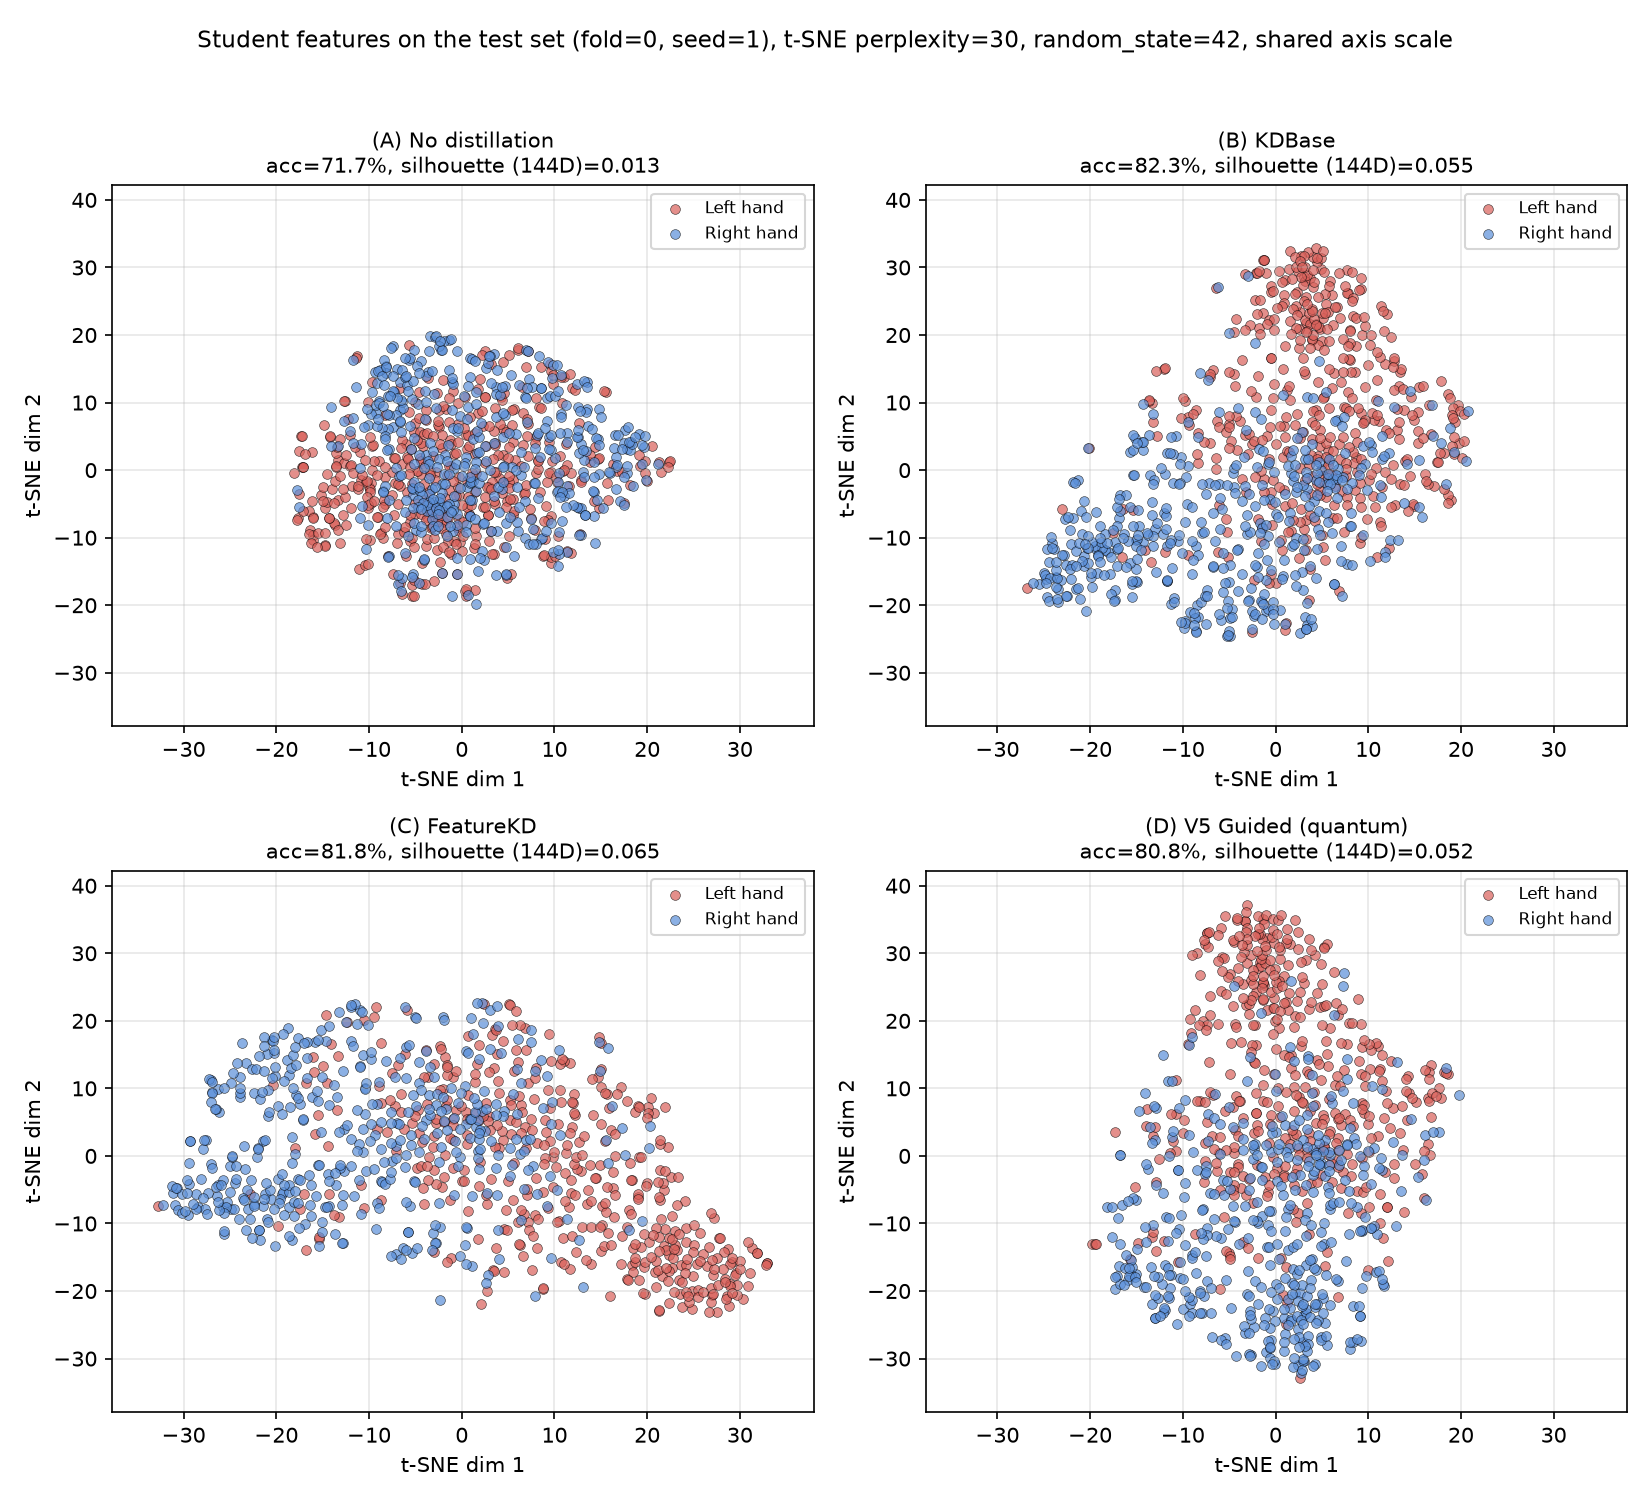
\includegraphics[width=\linewidth]{figs/image3_en.png}
\caption{Qualitative analysis of the feature space using t-SNE
visualization on the student's 144-dimensional intermediate
features, extracted on the test set at the epoch with the best
validation accuracy.}
\label{fig:tsne}
\end{figure}
\FloatBarrier

\paragraph{Qualitative analysis of the feature space (t-SNE)}

Figure~\ref{fig:tsne} visualizes the student's intermediate features
using t-SNE dimensionality reduction for four configurations: no
distillation, KDBase, FeatureKD, and V5 Guided (quantum kernel). All
four panels use the same fold (fold 0, 900 test samples, 20
subjects), the same training seed (seed 1), and the same t-SNE
hyperparameters (perplexity$=30$, random\_state$=42$). The accuracy
and silhouette score recorded in each panel's title belong to this
single run alone, not the 5-seed average used in the main tables.
The cluster structure of the three distilled configurations is more
clearly separated than the independent student (silhouette from
0.052 to 0.065, versus 0.013 for the no-distillation configuration).
This direction of difference agrees with the 6.56-percentage-point
accuracy gap measured over all 5 seeds above. Among the three
distilled configurations, the silhouette scores are close to one
another (0.052-0.065) even though the visually observed cluster
shapes differ. This is consistent with the finding of no detectable
systematic difference in the quantitative parts above. T-SNE is a
nonlinear projection that does not preserve global distances.
Therefore, visually observed differences in cluster shape are not
regarded as evidence of a real structural difference. The silhouette
index on the original 144-dimensional space is the quantitative
basis, while the figure is only illustrative.

\paragraph{Co-adaptation of the shared circuit parameters ($\theta$)}

Because $\theta$ is shared by both the teacher branch and the
student branch, a natural question arises. Could training shift
$\theta$ to make the two relation matrices easier to match (for
example, by making both kernels flatter), instead of genuinely
forcing the student to reproduce the exact relation structure that
the teacher has learned? To check this, the V2 Dense variant was
trained further under two other ways of handling $\theta$, different
from the current shared approach. The first keeps $\theta$ entirely
fixed (\emph{shared\_fixed}, $81.73\pm0.49\%$). The other separates
a fixed $\theta_T$ from a trainable $\theta_S$ (\emph{split},
$81.35\pm0.87\%$). Each way uses 5 seeds $\times$ 5 folds on
PhysionetMI. Both are compared against the result of sharing $\theta$
as in the original configuration (\emph{shared}, $81.49\pm0.78\%$,
already reported in Table~\ref{tab:tongthe}). No pair among the
three treatments differs significantly ($p=0.143$ between
\emph{shared} and \emph{shared\_fixed}, $p=0.615$ between
\emph{shared} and \emph{split}, $p=0.215$ between
\emph{shared\_fixed} and \emph{split}; $n=5$, $df=4$). This result
does not prove that the degeneracy risk noted above does not occur
at all, but it finds no sign of a measurable effect on accuracy at
the scale examined.

\paragraph{Initialization of $W_T$}

$W_T$ is initialized with PyTorch's default distribution after
several other calls that consume random numbers within the same
global random number stream, so it is likely to differ across the
experiment's seeds, even though this is not a deliberate
experimental manipulation. The question that arises is how much
$W_T$ contributes to the seed noise observed in the quantum branch.
To check this, V2 Dense was retrained on PhysionetMI with $W_T$
fixed at a single value, while still sweeping all five seeds
$\times$ 5 folds as in the original configuration. The standard
deviation across the five seeds drops from $0.78$ to $0.51$
percentage points, while the mean accuracy does not differ
significantly from the original V2 Dense ($81.20\%$ versus
$81.49\%$, $p = 0.22$, $n=5$, $df=4$). A substantial but not
complete part of the seed noise observed in the quantum branch
therefore comes from $W_T$ changing with the global seed, not only
from randomization in training. This control does not measure the
difference across multiple different initializations of $W_T$ at
the same training seed, so it is not yet a complete sensitivity
analysis with respect to the specific $W_T$ projection.

\subsubsection{Seed noise and the stability of the method ranking}
\label{sec:xephang}

No relation variant or kernel function separated from KDBase in the
part above. Is this because the true difference among methods is
small, or because seed noise exceeds the detection capability of the
protocol? One way to quantify the degree of separation among methods
is to compare two sources of variation. The standard deviation of
the mean values across the twelve distillation mechanisms is 0.459
percentage points. The average standard deviation from changing the
random seed, within the same mechanism, is 0.750 percentage points.
The ratio between the two quantities is 0.61. Among the twelve
mechanisms, FeatureKD is the only case with a statistically
significant effect relative to KDBase, so this mechanism alone
contributes 75\% of the total sum of squared deviations among the
twelve mean values. Excluding FeatureKD, the standard deviation
across the remaining eleven mechanisms drops to 0.205 percentage
points. The seed standard deviation for the same group is 0.726
percentage points. The ratio drops to 0.28. The gap among methods is
smaller than the noise that the training procedure itself generates.
This degree of separation becomes even clearer when the one
mechanism already known to have a real effect is set apart from the
rest.

A direct consequence of this noise level is a question: does the
method ranking drawn from a single run correctly reflect the true
order? Table~\ref{tab:daohang} compares the ranking obtained from a
single run with the ranking obtained from five seeds. The left
column corresponds to the common reporting protocol, in which a
configuration is run once across multiple folds, using the fixed
seed $20200220$. This is the default value in the training code,
fixed before the five-seed analysis protocol was built, so it is
not a choice made after seeing the results. The right column is
taken from 5 independent seeds.

\begin{table}[!htbp]
\centering
\caption{Effect of the number of random repetitions on the method
ranking (rank 6.5 = two tied configurations).}
\label{tab:daohang}
\begin{tabular}{lcccc}
\toprule
& \multicolumn{2}{c}{\textbf{One seed}} & \multicolumn{2}{c}{\textbf{Five seeds}} \\
\cmidrule(lr){2-3}\cmidrule(lr){4-5}
\textbf{Configuration} & Acc (\%) & Rank & Acc (\%) & Rank \\
\midrule
V2 Dense & 82.37 & \textbf{1} & 81.49 & 5.5 \\
V5 Guided & 81.86 & 2 & 81.12 & \textbf{11} \\
RBF kernel & 81.55 & 3 & 81.61 & 3.5 \\
Cosine kernel & 81.47 & 4 & 81.63 & 2 \\
V5 Guided ($\beta = 0.01$) & 81.40 & 5 & 81.47 & 7 \\
V4 Anchor+kNN & 81.32 & 6.5 & 81.42 & 8.5 \\
RelationalKD & 81.32 & 6.5 & 81.61 & 3.5 \\
V5 Guided ($\beta = 0.05$) & 81.21 & 8 & 81.42 & 8.5 \\
V3 Anchor & 81.14 & 9 & 81.25 & 10 \\
KDBase & 81.12 & 10 & 81.49 & 5.5 \\
V1 Dense & 81.06 & 11 & 81.90 & \textbf{1} \\
FeatureKD & 80.71 & 12 & 80.05 & \textbf{12} \\
\bottomrule
\end{tabular}
\end{table}
\FloatBarrier

The two rankings are nearly uncorrelated. The Spearman rank
correlation coefficient is $\rho = 0.14$ with $p = 0.66$. With only
twelve configurations, this result is not sufficient grounds to
reject the hypothesis of no relationship. The correlation
coefficient itself is also too weak to indicate a real relationship.
The ranking from a single run is almost unable to predict the
ranking from five seeds. The most dramatic rank reversal is V1
Dense, standing second-to-last, rank 11 out of 12, in the single
run, but rising to first place when computed over five seeds. V5
Guided goes in the opposite direction, standing second by the single
run but falling to second-to-last, eleven out of twelve, when
computed over five seeds.

If a single seed is unreliable, the next question is whether five
seeds are enough for the ranking to converge. Table~\ref{tab:hoitu}
directly checks this using the cumulative ranking over the first $k$
seeds, within the exact five seeds used for the main comparison.
Unlike the ``One seed'' column in Table~\ref{tab:daohang} (which
uses the fixed default seed $20200220$), $k=1$ here uses the first
of the five seeds 1--5, a different, independent data point
illustrating the same instability phenomenon.

\begin{table}[!htbp]
\centering
\caption{Spearman rank correlation between the cumulative ranking
over the first $k$ seeds and the final ranking ($k=5$).}
\label{tab:hoitu}
\begin{tabular}{cccc}
\toprule
$k$ & $\rho$ vs.\ $k=5$ & $p$ & $\rho$ vs.\ $k-1$ \\
\midrule
1 & 0.615 & 0.033 & --- \\
2 & 0.692 & 0.013 & 0.930 \\
3 & 0.853 & $<0.001$ & 0.895 \\
4 & 0.916 & $<0.001$ & 0.958 \\
5 & 1.000 & $<0.001$ & 0.916 \\
\bottomrule
\end{tabular}
\end{table}
\FloatBarrier

The correlation with the final ranking increases monotonically with
$k$, from $\rho=0.615$ at $k=1$ to $\rho=0.916$ at $k=4$, showing a
clear convergence trend. However, the correlation between the
second-to-last and last steps, $k=4$ versus $k=5$, adding exactly
one seed, still reaches only $\rho=0.916$, not $1.0$. Therefore,
five seeds are not necessarily the point of absolute convergence.
This result does not weaken the main point of this part; rather, it
adds further evidence for it. Seed noise is large enough that even
the ranking over four seeds does not fully predict the ranking over
five.

To check beyond the $k=5$ level, the study ran five additional new
seeds (6--10) for a subset of five mechanisms: KDBase, RelationalKD,
cosine (V5), V1 Dense, and the quantum kernel function (V5). With
only five mechanisms, the Spearman correlation coefficient has
coarse resolution, taking only a few discrete values, so the result
needs to be read together with the specific ranking order rather
than the $\rho$ figure alone. The correlation between the rankings
at $k=5$ and $k=10$ is $\rho=0.70$ ($p=0.19$), but it does not
increase monotonically with $k$ as in Table~\ref{tab:hoitu}.
Specifically, the three top mechanisms at $k=5$, V1, cosine, and
RelationalKD, swap order among themselves when extended to $k=10$,
with RelationalKD rising to first place and V1 dropping to second.
The two bottom mechanisms, KDBase and the quantum kernel function,
keep the same fourth and fifth positions throughout from $k=1$ to
$k=10$. Therefore, ranking instability does not stop at five seeds
for mechanisms with close results, even though the ranking of the
strongest and weakest mechanisms in this group is relatively stable
over time.

Because seeds are independent draws, the ranking from a single run
can be viewed as a prediction of the outcome when the experiment is
repeated. In that sense, this prediction is not reliable. The
correlation is positive but weak and not statistically significant,
and the position of each individual configuration can shift by many
ranks. The only configuration that keeps roughly the same position
at the bottom of the table is FeatureKD. That is also the only
configuration with an effect exceeding the noise floor.

Similar seed noise also affects the no-distillation configuration,
although here the sensitivity to the seed has an additional cause.
At $\alpha = 1.0$ (the value used for the main baseline), this
configuration has a standard deviation across seeds of 2.30
percentage points, about four times higher than the distilled
configurations. At $\alpha = 0.5$, this standard deviation rises to
5.03 points, about eight times higher (Table~\ref{tab:alphasweep}).
A configuration with unusually large variance across seeds relative
to the rest is a methodologically suspicious sign. In this case,
that very sign is what led to the $\alpha$-sensitivity survey
presented in Section~\ref{sec:hieuqua}.

\subsubsection{Evaluating the variants from a control-oriented perspective}
\label{sec:danhgiadk}

This part evaluates the variants from a control-oriented
perspective, using information transfer rate and the inference-time
budget instead of classification accuracy alone, to reach a specific
verdict for the quantum kernel function.

\begin{table}[!htbp]
\centering
\caption{Training cost of the distillation mechanisms, measured by
the average time per epoch.}
\label{tab:chiphi}
\begin{tabular}{lccc}
\toprule
\textbf{Mechanism} & \textbf{Time/epoch (s)} & \textbf{Multiple} & $\boldsymbol{\Delta}$ \textbf{Acc} \\
\midrule
KDBase & 1.05 & 1.0$\times$ & -- \\
RelationalKD & 1.10 & 1.0$\times$ & $+0.12$ ($p = 0.75$) \\
Cosine kernel & 1.10 & 1.0$\times$ & $+0.14$ ($p = 0.61$) \\
RBF kernel & 1.09 & 1.0$\times$ & $+0.13$ ($p = 0.51$) \\
V5 Guided & $\approx$13.6 & \textbf{$\approx$13}$\boldsymbol{\times}$ & $-0.37$ ($p = 0.23$) \\
V2 Dense & $\approx$13.6 & \textbf{$\approx$13}$\boldsymbol{\times}$ & $+0.00$ ($p = 1.00$) \\
\bottomrule
\end{tabular}
\end{table}
\FloatBarrier

Table~\ref{tab:chiphi} places training cost alongside the change in
accuracy, measured on the same NVIDIA H100 GPU. The ``$\approx$''
values are the average time from a single run, without a standard
deviation across repetitions, because no repeated-measurement data
is available for this. The classical distillation mechanisms,
including the cosine and RBF kernel functions, have nearly equal
training times at about 1.1 seconds per epoch. The variants using
the quantum kernel function require about 13.6 seconds per epoch,
about 13 times more, because the data re-uploading structure in
\eqref{eq:layer}--\eqref{eq:state} requires more circuit-simulation
passes per sample in the subsample than a single-pass
encode-then-entangle circuit.

A preliminary survey measures training cost as a function of the
number of qubits ($n_{\text{qubits}} \in \{4, 8, 12, 16\}$, keeping
every other hyperparameter fixed, 1 fold, 3 epochs, measuring time
only, not accuracy) using the V2 Dense configuration.
Table~\ref{tab:chiphi} shows that V2 and V5 Guided have the same
measured cost ($\approx 13\times$), because both select the same
number of sample pairs for the kernel function
(Table~\ref{tab:bienthe_cauhinh}, column Pair set $\mathcal{I}$:
``full $q\times q$'' for V2, ``teacher top-$q$'' for V5), differing
only in the pair-selection criterion, not in the number of pairs.
Because the number of qubits only affects the cost of each kernel
evaluation (the statevector size $2^{n_{\text{qubits}}}$), a
quantity that does not depend on the pair-selection criterion, the
trend measured on V2 has grounds to be extrapolated to V5 and the
other variants. This conclusion applies only to cost, not to the
accuracy of the main comparison on V5, which has not been
re-measured at these qubit levels.

\begin{table}[!htbp]
\centering
\caption{Training cost and accuracy as a function of the number of
qubits (V2 Dense). Time/epoch measured in the preliminary survey (1
fold $\times$ 3 epochs); accuracy measured in full (5 seeds $\times$
5 folds $\times$ 30 epochs) for $n_{\text{qubits}} \le 12$.}
\label{tab:qubitcost}
\footnotesize
\begin{tabular}{ccccc}
\toprule
$\boldsymbol{n_{\text{qubits}}}$ & \textbf{Time/epoch (s)} & \textbf{Multiple vs.\ previous level} & \textbf{Accuracy (\%)} & $\boldsymbol{p}$ \textbf{(vs.\ $n=4$)} \\
\midrule
4  & $\approx 13.6$ & -- & $81.49 \pm 0.78$ & -- \\
8  & 36--40 & $\approx 2.8\times$ & $81.36 \pm 0.38$ & $0.691$ \\
12 & 67--71 & $\approx 1.8\times$ & $81.16 \pm 0.75$ & $0.332$ \\
16 & 308--315 & $\approx 4.5\times$ & not measured (3 epochs not completed) & -- \\
\bottomrule
\end{tabular}
\end{table}
\FloatBarrier

Table~\ref{tab:qubitcost} shows that cost increases superlinearly
with the number of qubits, but the measured multiple between
consecutive levels (about $2.8\times$, $1.8\times$, and $4.5\times$
for each 4-qubit increase) is much lower than the $16\times$ that
statevector-simulation theory ($2^{n_{\text{qubits}}}$) predicts for
the quantum circuit part alone at the same increase. This gap
suggests that at the 4--16-qubit scale surveyed, the fixed cost of
the measurement (data loading, propagation through the classical
backbone, PennyLane function-call overhead) still accounts for a
substantial share, so the observed multiple does not yet fully
reflect the theoretical $2^{n_{\text{qubits}}}$ increase of the
circuit simulation alone. At $n_{\text{qubits}}=16$, the measurement
did not complete 3 epochs within the 20-minute budget allotted for
the preliminary survey. Extrapolating from this, a full training run
(5 seeds, 5 folds, 30 epochs) at this level would take about 65
hours for one configuration, far beyond the capacity of the current
shared single-GPU infrastructure. At $n_{\text{qubits}} \in \{8,
12\}$, the estimated cost is much lower (about 8 and 14 hours
respectively for one configuration), so the full survey was carried
out for V2 Dense at these two levels, with the resulting accuracy
presented in the table above. No pair among the three qubit levels
differs significantly, including the 8-versus-12 pair ($p=0.491$;
paired $t$-test over 5 seeds, $n=5$, $df=4$). With $n=5$, these
tests have low power, so this result only reflects that a trend
with the number of qubits has not been detected, not evidence
confirming that such a trend does not exist.

This cost increase is not accompanied by any measurable improvement
in accuracy, at least for V2. This cost arises only at the training
stage. The deployed model remains the classical student, with the
same number of parameters and the same inference time across every
configuration. Even so, for a realistic development process that
requires repeated retraining when adding data or tuning
hyperparameters, a factor of about 13 is a substantial cost.

\begin{table}[!htbp]
\centering
\caption{Control-oriented quantities derived from decoding accuracy,
via \eqref{eq:itr-bits}--\eqref{eq:itr-rate}.}
\label{tab:dieukhien}
\small
\begin{tabular}{lccc}
\toprule
\textbf{Configuration} & \textbf{Acc (\%)} & $\boldsymbol{B}$ \textbf{(bit/command)} & \textbf{Offline ITR (bit/min)} \\
\midrule
No distillation & 74.93 & 0.188 & 3.75 \\
\midrule
KDBase & 81.49 & 0.309 & 6.18 \\
FeatureKD & 80.05 & 0.279 & 5.58 \\
RelationalKD & 81.61 & 0.311 & 6.23 \\
\midrule
V1 Dense, deterministic dimensionality reduction & 81.90 & 0.318 & 6.35 \\
V2 Dense, learned projection & 81.49 & 0.309 & 6.18 \\
V3 Anchor & 81.25 & 0.304 & 6.08 \\
V4 Anchor $+$ kNN & 81.42 & 0.307 & 6.15 \\
V5 Guided & 81.12 & 0.301 & 6.02 \\
\midrule
Cosine kernel & 81.63 & 0.312 & 6.24 \\
RBF kernel & 81.61 & 0.312 & 6.23 \\
\bottomrule
\end{tabular}
\end{table}
\FloatBarrier

Following the control-oriented criteria noted in
Section~\ref{sec:rangbuoc}, Table~\ref{tab:dieukhien} converts
accuracy into operational quantities. For the balanced two-class
problem, $\kappa = 2\,acc - 1$ is a deterministic linear
transformation of accuracy that carries no additional information
and can be derived directly from the Acc column. For this reason,
the $\kappa$ coefficient is not listed in the table.

ITR is a monotonic transformation of accuracy at a fixed window
length (\eqref{eq:itr-bits}--\eqref{eq:itr-rate}), not an
independent measurement of the control system. The ITR increase
below therefore reflects exactly the accuracy increase already
reported in Section~\ref{sec:hieuqua}, not additional empirical
evidence. The bit/minute unit is still more useful than percent
accuracy for comparison against the control loop's budget. This is
the offline ITR, computed using $T_{\mathrm{window}}$ in
\eqref{eq:latency}. This value does not yet add $T_{\mathrm{infer}}$
(measured in Table~\ref{tab:tre}, under 1\% of $T_{\mathrm{window}}$
and therefore with negligible effect on ITR) or $T_{\mathrm{command}}$
(not yet measured, because the study is not tied to a specific
actuator). The online ITR of a complete control loop is therefore
lower than the values below, by an amount depending on
$T_{\mathrm{command}}$ of the specific deployed system.

With a signal window length of $T = 3.0$ s, the non-distilled
student gives an information transfer rate of 3.75 bit/min, while
every distilled configuration lies between 5.58 and 6.35 bit/min.
Corresponding to the reported accuracy increase, the control-channel
bandwidth increases by about 1.6 times relative to KDBase. Across
all ten configurations, including V1 Dense (the highest ITR value in
the table), the gap among distillation mechanisms is 0.77 bit/min,
coming largely from FeatureKD alone. If this configuration is
excluded, the gap narrows to 0.33 bit/min, corresponding to about
5.4\% of the bandwidth and of no operational significance.

Table~\ref{tab:tre} decomposes the time budget of the closed loop.
Inference time is measured on the CPU of a shared compute node of
the HPC cluster, with batch size one, taking the median and 95th
percentile over 200 runs after 20 warm-up runs. Hardware and
software configuration: AMD EPYC 9224 CPU (24 cores per socket, 2
sockets, max clock $\approx 3.7$ GHz), 8 threads (the default
number of CPUs allocated to the measurement process, not specially
tuned for this measurement), PyTorch $2.7.1$, Intel oneAPI MKL BLAS
backend (PyTorch's default, not specially optimized for the AMD
architecture), float32 precision, Linux kernel 5.14 operating system
(Enterprise Linux 9). The hardware and software configuration was
confirmed to be on the same compute node, although it does not rule
out the possibility of a slight change in OS patches between
measurements on the shared infrastructure.

\begin{table}[!htbp]
\centering
\caption{Decomposition of the closed control loop's time and
resource budget via \eqref{eq:latency}, measured on the HPC server
CPU and on a Raspberry Pi 4.}
\label{tab:tre}
\begin{tabular}{lcc}
\toprule
\textbf{Component} & \textbf{Student (EEGNet)} & \textbf{Teacher (Ensemble-MI)} \\
\midrule
Number of parameters & 2,402 & $15.1$ K \\
$T_{\mathrm{window}}$ & 3000 ms & 3000 ms \\
\midrule
\multicolumn{3}{l}{\textit{HPC server CPU}} \\
$T_{\mathrm{infer}}$ (median) & 3.17 ms & 22.38 ms \\
$T_{\mathrm{infer}}$ (p95) & 3.31 ms & 22.63 ms \\
Ratio of $T_{\mathrm{infer}}$ to $T_{\mathrm{window}}$ & 0.11\% & 0.75\% \\
MACs per inference (batch=1) & $\approx 10.2$ million & not computed \\
Peak activation (fp32, batch=1) & $\approx 600$ KB & not computed \\
Precision & float32 & float32 \\
\midrule
\multicolumn{3}{l}{\textit{Raspberry Pi 4, ARM Cortex-A72 (mean
$\pm$ standard deviation over 5 independent runs)}} \\
$T_{\mathrm{infer}}$ (median) & $7.99 \pm 0.08$ ms & $85.30 \pm 1.42$ ms \\
$T_{\mathrm{infer}}$ (p95) & $8.14 \pm 0.11$ ms & $87.26 \pm 1.48$ ms \\
Ratio of $T_{\mathrm{infer}}$ to $T_{\mathrm{window}}$ & 0.27\% & 2.84\% \\
RAM after loading the model (RSS) & $216.08 \pm 0.03$ MB & $219.11 \pm 0.05$ MB \\
Peak RAM during inference (RSS) & $238.07 \pm 0.02$ MB & $251.63 \pm 0.11$ MB \\
\bottomrule
\end{tabular}
\end{table}
\FloatBarrier

The student has a median
$T_{\mathrm{infer}}$ of 3.17 ms and the teacher a median of 22.38
ms. Compared with the 3000 ms signal window, these two components
occupy 0.11\% and 0.75\% of the budget, respectively. Both models
fall within the closed loop's time budget when run on a workstation,
so the real-time constraint by itself does not rule out the teacher.

The gap between the two models lies along a different dimension. The
teacher is 6.3 times larger than the student in parameter count and
7.1 times slower in inference time. On a workstation, this ratio
does not matter, because both are many orders of magnitude faster
than the signal window. On the hardware built into the device, the
tightening constraints are memory and energy. There, the sixfold
difference in model size becomes significant. The $T_{\mathrm{infer}}$
values just noted are measured on the CPU of the high-performance
computing system, not on a microcontroller or the target embedded
hardware. The student's 3.17 ms value is on the same order of
magnitude as the 2.95 ms reported by another EEGNet deployment on an
ultra-low-power microcontroller \cite{wang2024mibminet}. These are
two different architectures, two different datasets, and two
different types of hardware, so the similarity in CPU inference time
does not prove that the two models have equivalent deployment
conditions. Inference time on an MCU also depends on the number of
MACs, intermediate RAM (activation), precision, the kernel library,
and the specific MCU type, not just the parameter count or the time
measured on a CPU. The MACs and peak activation in
Table~\ref{tab:tre} are computed analytically directly from the
EEGNet architecture, not measured on hardware, and are reported only
for the student, since this is the deployed model. For the student,
the analytically estimated peak activation is about 600 KB at
float32 precision, larger than the total RAM of many low-end
microcontroller families (typically a few tens to a few hundred KB).
Therefore, the current architecture has deployment potential but has
not been confirmed feasible on every class of embedded hardware. A
definitive conclusion requires direct measurement on the target
hardware or further optimization of intermediate memory (for
example, reducing precision, or processing smaller channel batches).

An additional measurement on real embedded hardware narrows part of
this gap. On a Raspberry Pi 4 (ARM Cortex-A72, 64-bit, no GPU), the
same student and teacher architectures are exported with TorchScript
and measured following exactly the same protocol used for the HPC
server CPU part in Table~\ref{tab:tre} (200 inferences after 20
warm-up runs, batch size one, no special thread-count
configuration). The measurement is repeated over 5 independent runs,
following the paper's own 5-repetition convention, and is
re-verified with a second independent measurement pass that gives
results consistent within error. The lower part of Table~\ref{tab:tre}
summarizes this result.

For the student, the median $T_{\mathrm{infer}}$ is $7.99 \pm 0.08$
ms and the 95th percentile is $8.14 \pm 0.11$ ms, about $2.5$ times
higher than on the HPC server CPU, but occupying only about
$0.27\%$ of the 3000 ms signal-window budget. Latency ranges from
$7.6$ to $10.0$ ms across all measurements, with the hardware
confirmed to be free of thermal throttling ($39.4^\circ$C, no
throttling, CPU frequency held at the maximum 1800 MHz throughout the
measurement). An earlier measurement session on the same device
(with no record of thermal state or background load at the time of
measurement) gave slower results with much wider variation (median
$26.68 \pm 3.24$ ms), consistent with the hypothesis that latency on
this low-cost embedded hardware is sensitive to instantaneous
operating conditions (CPU frequency scaling, background load,
temperature), not just to the model architecture.

For the teacher, the median $T_{\mathrm{infer}}$ is $85.30 \pm 1.42$
ms, about $10.7$ times higher than the student on the Pi 4, compared
with about $7.1$ times measured on the HPC server CPU
(Table~\ref{tab:tre}). The gap between the two models therefore
widens further on weaker hardware rather than keeping the same
ratio, consistent with the argument noted above that memory and
energy constraints on embedded hardware make the scale difference
between the two models more significant than on a workstation. Even
so, $85.30$ ms still occupies only about $2.84\%$ of the 3000 ms
budget, so the teacher's inference time by itself is not the main
deployment barrier on this device. The real barrier lies in memory.
The teacher's peak RAM ($251.63 \pm 0.11$ MB) is only about $5.7\%$
higher than the student's, even though the teacher has $6.3$ times
as many parameters, because most of the RAM measured for both models
comes from the fixed overhead of the Python interpreter and the
PyTorch runtime, not from the model's actual weights or activations.
This is the RAM of the entire process, fundamentally different from
the analytically estimated $\approx 600$ KB of pure student
activation in Table~\ref{tab:tre}, and these two figures should not
be compared directly. This measurement uses randomly initialized
weights instead of trained weights, because inference time and
memory usage depend only on the architecture and tensor sizes, not
on the weight values. The Raspberry Pi 4 does not belong to the
ultra-low-power microcontroller class as in \cite{wang2024mibminet}.
This result therefore does not yet confirm feasibility on the lowest
tier of hardware, but it is the first direct measurement evidence in
the paper on real embedded hardware, rather than an inference from a
workstation CPU alone.

The implication for system design is fairly clear. Applying
knowledge distillation provides a large and measurable benefit for
control-channel bandwidth (measured by offline ITR,
Table~\ref{tab:dieukhien}). Within the scope of the configurations
surveyed, the difference among distillation mechanisms in this
bandwidth is small (0.77 bit/min, coming largely from FeatureKD
alone, and 0.33 bit/min if this configuration is excluded) and not
large enough to be operationally meaningful. Therefore, the
reasonable selection criterion is training cost and implementation
complexity. With the current implementation, the roughly 13-fold
cost of the quantum branch is not accompanied by a measurable
benefit, so a cheaper distillation mechanism is the practical
choice. This statement is limited to the quantum configuration
surveyed and does not extend to other implementations.

\section{Conclusion}
\label{sec:ketluan}

This paper presents a controlled survey of the role of relation
structure and representation space in knowledge distillation,
applied to motor imagery decoders, evaluated offline under
control-loop constraints, on PhysionetMI and the two-class
discrimination problem. This framework keeps the relation kernel
function, whether classical or quantum, participating only in the
training stage, so the deployed model retains the inference cost of
a lightweight classical network. Five relation-formation strategies
and three kernel function types were compared under uniform
conditions, with the seed as the statistical unit over 5 independent
seeds. Besides the QRD framework, the paper also proposes a
control-oriented evaluation procedure, using information transfer
rate and the inference-time budget instead of classification
accuracy alone, applied consistently across every configuration and
illustrated with a real inference-time measurement on embedded
hardware.

Overall, the main picture of the study consists of two complementary
parts. Knowledge distillation creates a large and replicable gap
relative to an independently trained student, on both datasets. But
once distillation is present, the choice of specific mechanism
hardly matters anymore. The difference among the twelve distillation
configurations lies within the natural noise margin of the training
process, large enough to reverse the method ranking between runs.
The only mechanism that separates, FeatureKD, gives an effect close
to the protocol's own minimum detectable threshold (about 1.4
percentage points), so this is not simply a lack of statistical
power. The quantum circuit, surveyed as the strictest test case for
the second finding, is no exception. It does not separate from the
two classical kernel functions in accuracy, while requiring a
training cost higher by one order of magnitude (about 13 times). The
conclusion about the quantum circuit is limited to the specific
implementation surveyed.

Two design consequences follow, within the scope of the problem
surveyed. The choice of specific distillation mechanism changes the
control-channel bandwidth by only 0.77 bit/min, mostly due to
FeatureKD alone. This magnitude of change is not enough to be
operationally meaningful. The reasonable selection criterion is
therefore training cost and implementation complexity, not accuracy.
For the quantum kernel function, both the original test and the two
additional cross-check methods place the difference from cosine in
the same ambiguous region. This region sits right at the
pre-specified equivalence margin of $\pm 0.5$ percentage points.
None of these readings establishes either equivalence or a
significant difference. This is a quantitative benchmark for
comparison when more complex quantum configurations are tested
later.

The study has several limitations that need to be stated clearly.
The main comparison is carried out only on PhysionetMI. The survey
on Cho2017 is exploratory and cannot substitute for it. The Cohen's
kappa coefficient does not provide much additional information
beyond accuracy in this balanced two-class problem. The study has
not measured per-subject $F_1$ to quantify the possible difference
between the two metrics. The quantum component is implemented in
only one specific circuit form (four qubits, data re-uploading, run
on a simulator), so the conclusion does not extend to quantum
machine learning in general. Several design assumptions, including
sharing the circuit weights $\theta$ between the teacher and
student, the initialization of the projection $W_T$, sharing the
coefficient $\beta$ across the three kernel function types, and the
different candidate pool between V5 and V2--V4, have been checked
with experimental controls in Section~\ref{sec:chuyensau}. None of
the controls entirely rules out the corresponding theoretical risk,
although the fixed-$W_T$ control shows that a substantial part of
the seed noise in the quantum branch comes from this very
initialization.

Directions for future work include repeating the main comparison,
with a statistical protocol and equivalence margin fixed before
running, on the second dataset instead of stopping at an exploratory
survey; extending to the multi-class problem, where there is more
room for improving the information transfer rate; and completing
the accuracy survey for V5 rather than only V2, at a larger number
of qubits or deeper entangling layers ($n_{\text{qubits}}=16$ is not
yet feasible in cost on the current infrastructure). On the
methodological front, building a protocol that determines the
minimum number of random repetitions, based on the measured noise
floor, would help make method comparisons in this field more
reliable.

\textbf{Reproducibility.} The training, preprocessing, and
statistical analysis code used in the paper, together with the
complete list of subject-to-fold assignments (515 entries), will be
made publicly available at
\url{https://github.com/nguyenphuonghuy/qrd_eeg} after the paper is
accepted. Beyond the released code, reproducibility also rests on
four factors
described in detail in the paper: a version-pinned software
environment (PyTorch 2.7.1, PennyLane, braindecode), the two public
datasets PhysionetMI and Cho2017, five fixed random seeds fully
listed for every comparison, and a preregistered statistical
analysis protocol that did not change after seeing the results.

\section*{Acknowledgments}

The authors would like to thank the High-Performance Computing
Laboratory, Thai Nguyen University of Technology (TNUT), for
supporting this research.


\bibliographystyle{IEEEtran}
\bibliography{references}

\end{document}
